%%%%%%%%%%%%%%%%%%%%%%%%%%%%%%%%%%%%%%%%%%  不使用 authblk 包制作标题  %%%%%%%%%%%%%%%%%%%%%%%%%%%%%%%%%%%%%%%%%%%%%%
%-------------------------------PPT Title-------------------------------------
\title{赝势、投影函数与\rm{VASP}的\rm{POTCAR}}
%-----------------------------------------------------------------------------
%----------------------------Author & Date------------------------------------

%\author[\textrm{Jun\_Jiang}]{姜\;\;骏\inst{}} %[]{} (optional, use only with lots of authors)
%% - Give the names in the same order as the appear in the paper.
%% - Use the \inst{?} command only if the authors have different
%%   affiliation.
\institute[BCC]{\inst{}%
%\institute[Gain~Strong]{\inst{}%
\vskip -20pt 北京市计算中心}
%\vskip -20pt {\large 格致斯创~科技}}
\date[\today] % (optional, should be abbreviation of conference name)
{%	{\fontsize{6.2pt}{4.2pt}\selectfont{\textcolor{blue}{E-mail:~}\url{jiangjun@bcc.ac.cn}}}
\vskip 45 pt {\fontsize{8.2pt}{6.2pt}\selectfont{%清华大学\;\;物理系% 报告地点
	\vskip 5 pt \textrm{2023.08.24}}}
}

%% - Either use conference name or its abbreviation
%% - Not really information to the audience, more for people (including
%%   yourself) who are reading the slides onlin%%   yourself) who are reading the slides onlin%%   yourself) who are reading the slides onlineee
%%%%%%%%%%%%%%%%%%%%%%%%%%%%%%%%%%%%%%%%%%%%%%%%%%%%%%%%%%%%%%%%%%%%%%%%%%%%%%%%%%%%%%%%%%%%%%%%%%%%%%%%%%%%%%%%%%%%%

\subject{}
% This is only inserted into the PDF information catalog. Can be left
% out.
%\maketitle
\frame
{
%	\frametitle{\fontsize{9.5pt}{5.2pt}\selectfont{\textcolor{orange}{“高通量并发式材料计算算法与软件”年度检查}}}
\titlepage
}
%-----------------------------------------------------------------------------

%------------------------------------------------------------------------------列出全文 outline ---------------------------------------------------------------------------------
%\section*{}
%\frame[allowframebreaks]
%{
%  \frametitle{Outline}
%%  \frametitle{\textcolor{mycolor}{\secname}}
%  \tableofcontents%[current,currentsection,currentsubsection]
%}
%%在每个section之前列出全部Outline
%%类似的在每个subsection之前列出全部Outline是\AtBeginSubsection[]
%\AtBeginSection[]
%{
%  \frame<handout:0>%[allowframebreaks]
%  {
%    \frametitle{Outline}
%%全部Outline中,本部分加亮
%    \tableofcontents[current,currentsection]
%  }
%}

%-----------------------------------------------PPT main Body------------------------------------------------------------------------------------
\small
%\section{\rm{VASP~}软件中\rm{PAW~}计算的实现}
%\frame
%
%	\frametitle{\textrm{VASP}计算的特色}
%	相比于与普通的第一原理计算软件,\textrm{VASP}很好地平衡了计算效率和精度的问题,总的来说,\textrm{VASP}主要通过这几个特色保证了计算的高效能
%	\begin{itemize}
%	     \item 迭代与优化算法的多样性\\
%		     本质上电荷密度迭代 \textrm{\&\&} 体系总能量优化是相同的优化问题,采用了类似的算法\upcite{CMS6-15_1996,PRB54-11169_1996}:\\
%			\textcolor{blue}{\textrm{Pseudo-Newton、Conjugate-Gradient、Broyden~mix、damping-factor、RMM-DIIS}}
%	     \item 尽可能采用局域基(原子轨道基)函数:~\\
%		     \textcolor{blue}{\textrm{LREAL}}=\textcolor{red}{\textrm{.TRUE.}}\\
%			优化的投影函数也尽可能在实空间表示
%	     \item \textrm{PAW}原子数据集:\textcolor{blue}{优异的赝势}\upcite{PRB59-1758_1999}
%	\end{itemize}
%}
\section{赝势理论}       %Bookmark
%\section{Induction on DFT and solid-state physics}       %Bookmark
\subsection{平面波与赝势}       %Bookmark
\frame
{
	\frametitle{球形势对平面波的散射与相移}
\begin{figure}[h!]
\centering
\vspace*{-0.26in}
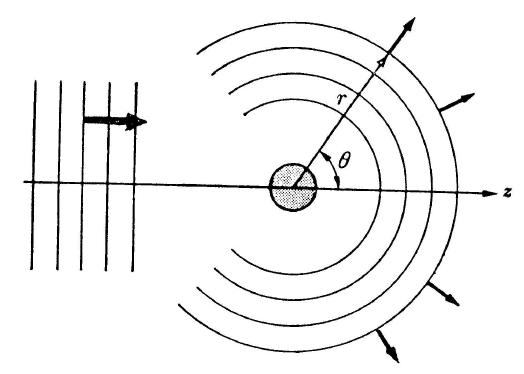
\includegraphics[height=0.90in,width=1.24in,viewport=0 0 400 300,clip]{Figures/Pseudo-scatter.jpg}
\caption{\fontsize{5.5pt}{4.2pt}\selectfont{\textrm{Schematic illustration of scattering of a plane wave by a spherical potential.}}}%(与文献\cite{EPJB33-47_2003}图1对比)
\label{Pseudo-scatter}
\end{figure}
\vspace*{-0.1in}
\fontsize{7.5pt}{6.2pt}\selectfont{
入射平面波
$$\mathrm{e}^{\mathrm{i}\vec q\cdot\vec r}=4\pi\sum_{lm}\mathrm{i}^lj_l(\vec q\cdot\vec r)Y_{lm}^{\ast}(\hat{\vec q})Y_{lm}(\hat{\vec r})=\sum_{l}(2l+1)\mathrm{i}^lj_l(qr)P_{l}(\cos\theta)$$
%$$\mathrm{e}^{\mathrm{i}\vec q\cdot\vec r}=\mathrm{e}^{\mathrm{i}qr\cos(\theta)}=\sum_{l}(2l+1)\mathrm{i}^lj_l(qr)P_{l}[\cos(\theta)]$$
经散射后出射,波函数变为
$$\Psi_l^{>}(\varepsilon,r)=C_l\bigg[j_l(\kappa r)-\tan\eta_l(\varepsilon)n_l(\kappa r)\bigg]\quad\text{其中}\kappa^2=\varepsilon$$
根据散射理论,能量为$\varepsilon$的电子经单个势阱散射偏转$\theta$后,波函数的振幅可以表示为
	\begin{displaymath}
		t(\theta)=\dfrac{4\pi}{\kappa}\sum_l(2l+1)[\mathrm{exp}(2\mathrm{i}\eta_l(\varepsilon))-1]P_l(\cos\theta)
	\end{displaymath}
%$$t(\theta)=\dfrac{4\pi}{\sqrt\varepsilon}\sum_l(2l+1)\bigg[\mathrm{e}^{2\mathrm{i}\eta_l(\varepsilon)}-1\bigg]P_l(\cos\theta)$$
%$$\eta_l(\varepsilon)=p_l\pi+\delta_l(\varepsilon)$$
}
}

\frame
{
	\frametitle{散射相移与赝势}
\begin{figure}[h!]
\centering
\vspace*{-0.20in}
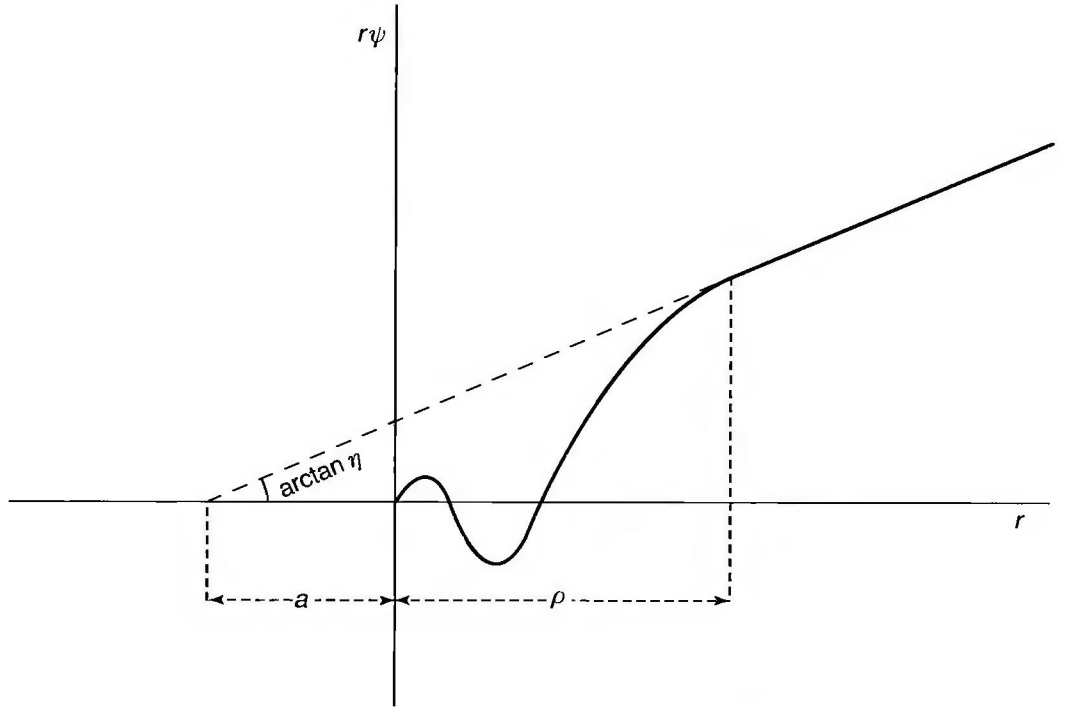
\includegraphics[height=1.20in,width=1.77in,viewport=0 0 1150 750,clip]{Figures/Pseudo-scatter-2.png}
\caption{\fontsize{4.5pt}{3.2pt}\selectfont{\textrm{Radial wave-function $\phi=r\psi$ for low-energy scattering as illustrated in a figure from the 1934 and 1935 papers of Fermi and coworkers for low-energy electron scattering from atoms and neutron scattering from nuclei. The node in the wave-function near the origin show that the potential is attractive and strong enough to have bound states. The cross-section for scattering from the localized potential is determined by the phase shift and is the same for weaker pseudo-potential with the same phase shift modulo $2\pi$.}}}%(与文献\cite{EPJB33-47_2003}图1对比)
\label{Pseudo-scatter-2}
\end{figure}
\fontsize{7.5pt}{6.2pt}\selectfont{
对于球形势散射,相移可由径向波函数计算
$$\tan\eta_l(\varepsilon)=\dfrac{R\frac{\mathrm{d}}{\mathrm{d}r}j_l(\kappa r)|_R-D_l(\varepsilon)j_l(\kappa R)}{R\frac{\mathrm{d}}{\mathrm{d}r}n_l(\kappa r)|_R-D_l(\varepsilon)n_l(\kappa R)}$$
$$\mbox{其中~}D_l(\varepsilon,r)\equiv r\psi_l^{\prime}(r)/\psi_l(r)=r\dfrac{\mathrm{d}}{\mathrm{d}r}\ln\psi_l(r)$$
同时相移与波函数节点的关系为:$$\eta_l(\varepsilon)=p_l\pi+\delta(\varepsilon)$$}
}

\frame
{
%\frametitle{The methods on band structure calculation}
	\frametitle{由\textrm{OPW~}到赝势}
%\vskip 10pt
%\textrm{The mainly difference of all these methods below: the basis sets and the construction of the potential}
\begin{itemize}
%\setlength{\itemsep}{5pt}
	\item 完全平面波基组\\{\fontsize{7.5pt}{5.5pt}\selectfont{少数平面波就可以很好地描述波函数在原子间的行为,近核波函数则需要大量平面波展开}}%。因此完全平面波基组虽然方便,但求体系本征态对角化的矩阵非常巨大,计算变得异常耗时。
	\item 正交平面波(\textrm{Orthogonalized plane wave, OPW})方法\\{\fontsize{7.5pt}{5.5pt}\selectfont{价电子波函数由芯电子波函数和平面波共同展开
		\begin{displaymath}
			\phi_{\mathrm{OPW}}^{\vec k+\vec G}(\vec r)=\phi_{\mathrm{PW}}^{\vec k+\vec G}(\vec r)-\sum_c\langle\varphi_c|\phi_{\mathrm{PW}}^{\vec k+\vec G}\rangle\varphi_c(\vec r)
		\end{displaymath}}}
	{\fontsize{7.5pt}{5.5pt}\selectfont{通过价电子和芯电荷波函数叠加构造赝波函数
		\begin{displaymath}
			\textcolor{blue}{\tilde{\phi}_v(\vec r)}=\textcolor{red}{\phi_v(\vec r)}+\sum_c\langle\varphi_c|\textcolor{blue}{\tilde{\phi}_v}\rangle\varphi_c(\vec r)
		\end{displaymath}
	代入\textrm{Schr\"odinger}方程
		$$\hat H|\tilde{\phi}_v\rangle-\sum_c\langle\varphi_c|\tilde{\phi}_v\rangle\hat H|\varphi_c\rangle=\varepsilon_v|\tilde{\phi}_v\rangle-\varepsilon_v\sum_c\langle\varphi_c|\tilde{\phi}_v\rangle|\varphi_c\rangle$$
		可有$$\hat H|\tilde{\phi}_v\rangle+\textcolor{blue}{V^R}|\tilde{\phi}_v\rangle=\textcolor{blue}{\varepsilon_v}|\tilde{\phi}_v\rangle$$
		这里排斥势是$$V^R(\vec r,\vec r^{\prime})=\sum_c(\varepsilon_v-\varepsilon_c)|\varphi_c(\vec r^{\prime})\rangle\langle\varphi_c(\vec r)|$$}}
\end{itemize}
}

\frame
{
	\frametitle{由\textrm{OPW~}到赝势}
	\textrm{Phillips-Kleinman}指出,赝势($V^{\mathrm {eff}}$)-赝波函数(可用$\phi_{\mathrm{PW}}^{\vec k+\vec G}$展开)满足\textrm{Schr\"odinger}方程%\upcite{PR116-287_1959}
	$$\bigg(-\dfrac12\nabla^2+\textcolor{red}{V^{\mathrm {eff}}}\bigg)|\tilde{\phi}_v\rangle=\textcolor{blue}{\varepsilon_v}|\tilde{\phi}_v\rangle$$
	其中$\textcolor{red}{V^{\mathrm {eff}}}=V(\vec r)+\textcolor{blue}{V^R}$
	\begin{itemize}
		\item 赝势-赝波函数的本征值$\varepsilon_v$与真实体系的价电子能量本征值\textcolor{purple}{相等}
		\item 赝势$\textcolor{red}{V^{\mathrm {eff}}}$比$V(\vec r)$平滑得多,并且$\textcolor{blue}{V^R}$是非局域的排斥势
			\begin{displaymath}
				\begin{aligned}
					\textcolor{blue}{V^R}f(\vec r)=&\sum_c(\varepsilon_v-\varepsilon_c)\varphi_c(\vec r)\int\varphi_c^{\ast}(\vec r^{\prime})f(\vec r^{\prime})\mathrm{d}\vec r^{\prime} \\
					=&\int V^R(\vec r,\vec r^{\prime})f(\vec r^{\prime})\mathrm{d}\vec r^{\prime}
				\end{aligned}
			\end{displaymath}
%			这里$$V^R(\vec r,\vec r^{\prime})=\sum_c(\varepsilon_v-\varepsilon_c)|\varphi_c(\vec r^{\prime})\rangle\langle\varphi_c(\vec r)|$$
	\end{itemize}
}

\frame
{
	\frametitle{\textrm{PK}型赝势}
	\textrm{Phillips-Kleinman~(PK)}赝势取为
	\begin{displaymath}
		\tilde{V}^{\mathrm{PK}}=V(\vec r)\textcolor{blue}{+\sum_c(\varepsilon_v-\varepsilon_c)|\varphi_c\rangle\langle\varphi_c|}
	\end{displaymath}
	对应的赝波函数可以表示为
	\begin{displaymath}
		|\tilde{\psi}^{\mathrm{PK}}\rangle=|\psi_t\rangle-\sum_c\langle\varphi_c|\psi_t\rangle|\varphi_c\rangle
	\end{displaymath}
	\textrm{PK}型赝势的一些不足
	\begin{itemize}
		\item 构造赝波函数时必须有与价电子正交的芯电子波函数:\\
			因此对于$1s$、$2p$、$3d$等轨道,无法实施\textrm{PK}型赝化方案
		\item 赝势$\tilde{V}^{\mathrm{PK}}$依赖于能量本征值$\varepsilon_v$:\\
			源于正交平面波的非正交归一性,导致构建的久期方程的非对角元项对能量依赖
		\item 与芯电荷区以外,赝波函数与价波函数的模不相等:\\
			每次计算后必须将波函数重新归一化
	\end{itemize}
}

\frame
{
\frametitle{赝势的评估}
赝势(\textrm{Pseudo Potential, PP})方法是在正交平面波的基础上发展起来的,构造出平缓的势函数代替核的强吸引作用和芯层电子的排斥作用,用平缓的函数取代波函数近核时的震荡。
\begin{itemize}
\setlength{\itemsep}{5pt}
	\item 赝势-平面波方法,只需要少量平面波可展开赝波函数,大大提升了计算效率;但是赝波函数不能很好地反映与电子近核行为有关的性质。
	\item 赝势的构造并不唯一,考核构造赝势的两大指标:~\\“柔软程度”\textrm{(Soft)}与“可移植性”\textrm{(transferability)}
\end{itemize}
\begin{figure}[h!]
\centering
\vspace*{-0.10in}
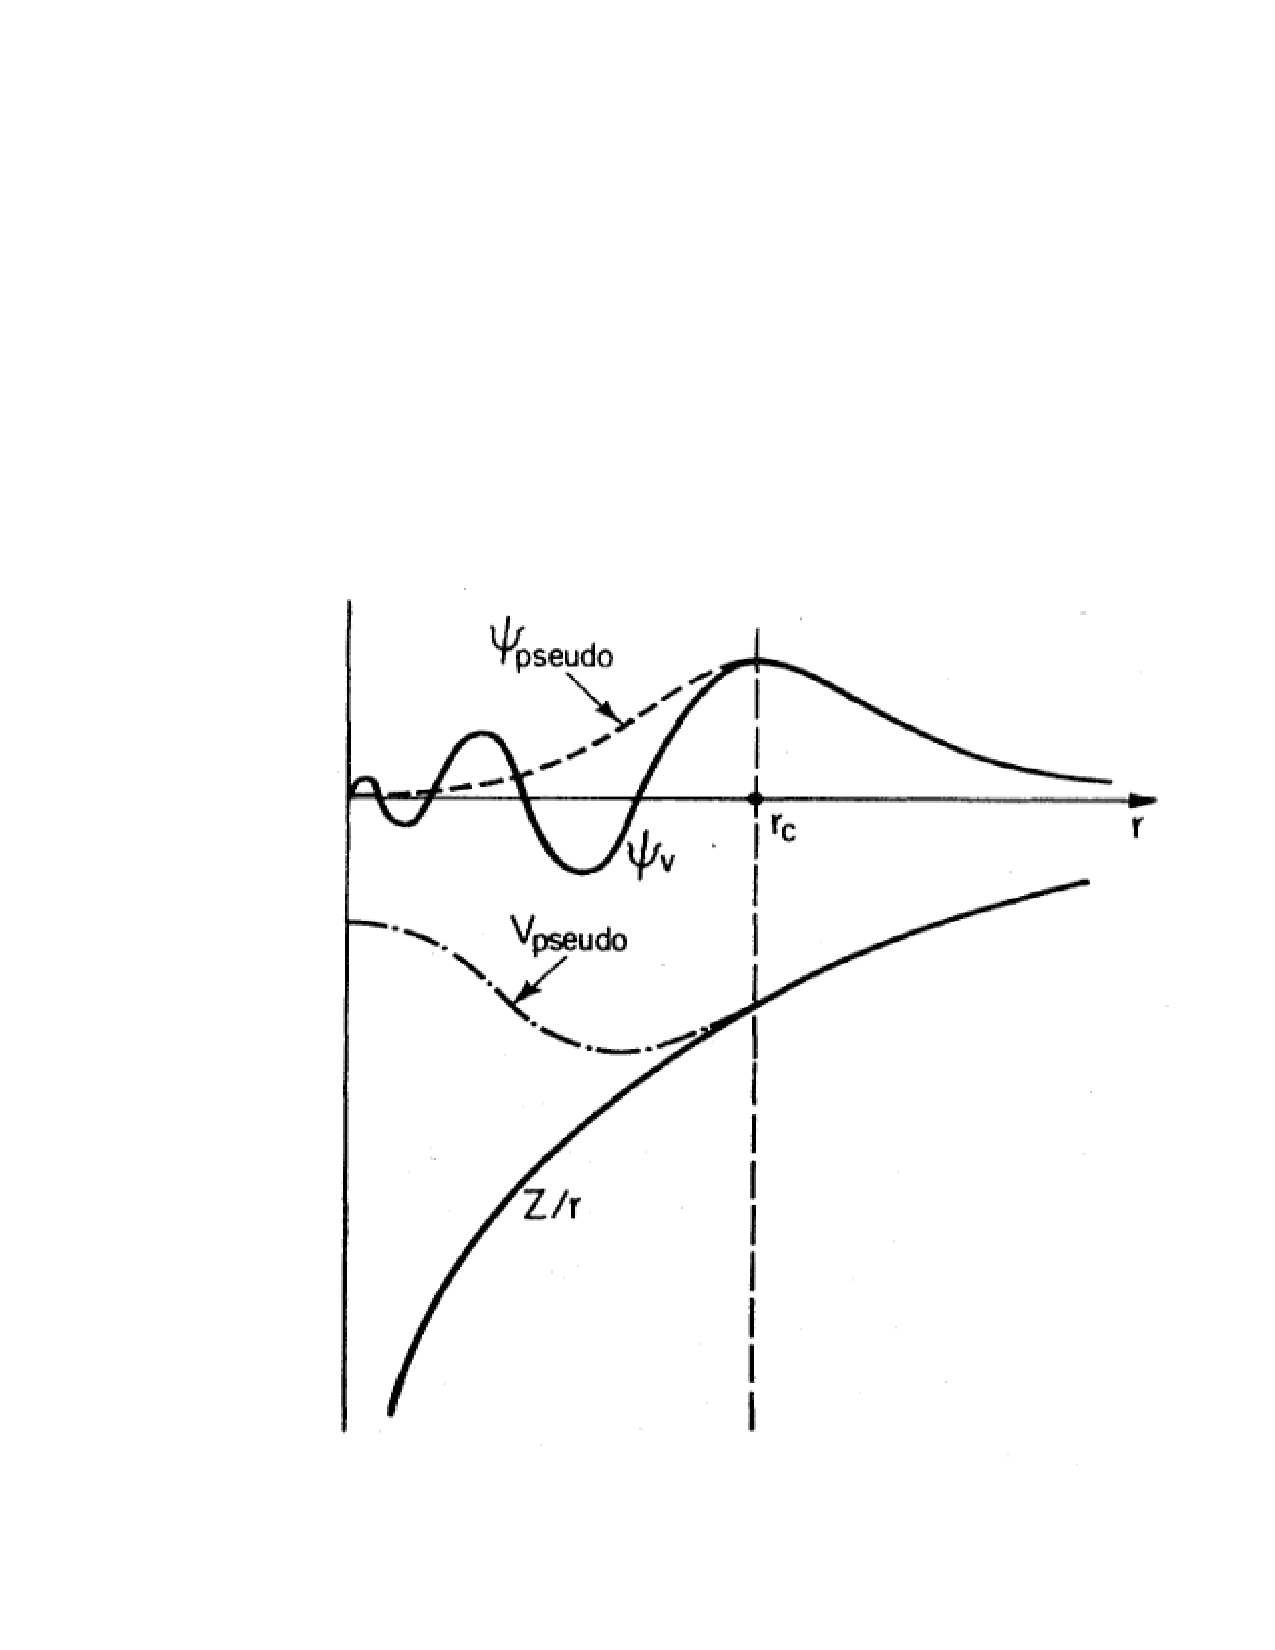
\includegraphics[height=1.35in,width=1.40in,viewport=154 100 562 508,clip]{Figures/Pseudo.pdf}
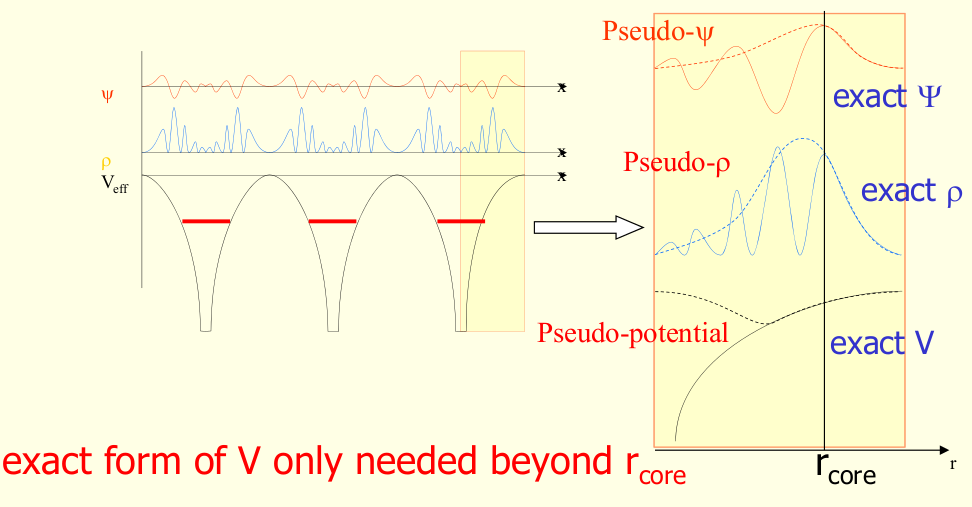
\includegraphics[height=1.35in,width=2.55in,viewport=1 1 980 500,clip]{Figures/Pseudo-2.png}
\caption{\tiny \textrm{The Pseudo wave function and Pseudo potential.}}%(与文献\cite{EPJB33-47_2003}图1对比)
\label{Pseudo_Potential-Wave}
\end{figure}
}

\subsection{模守恒赝势与超软赝势}
\frame
{
	\frametitle{传统赝势的构造}
	直接由实验数据来确定(模型)赝势,常用的实验数据包括离子对电子的散射角度、离子的光谱实验数据等
		\begin{itemize}
			\item 构造离子赝势:~可移植性好
			\item 构造总赝势(包括全部价电子相互作用):~常用于能带描述
		\end{itemize}
%	\begin{itemize}
%		\item 在指定能量范围内,离子对电子散射的散射角
%		\item 离子的光谱实验数据
%	\end{itemize}
\begin{figure}[h!]
\centering
\vspace*{-0.10in}
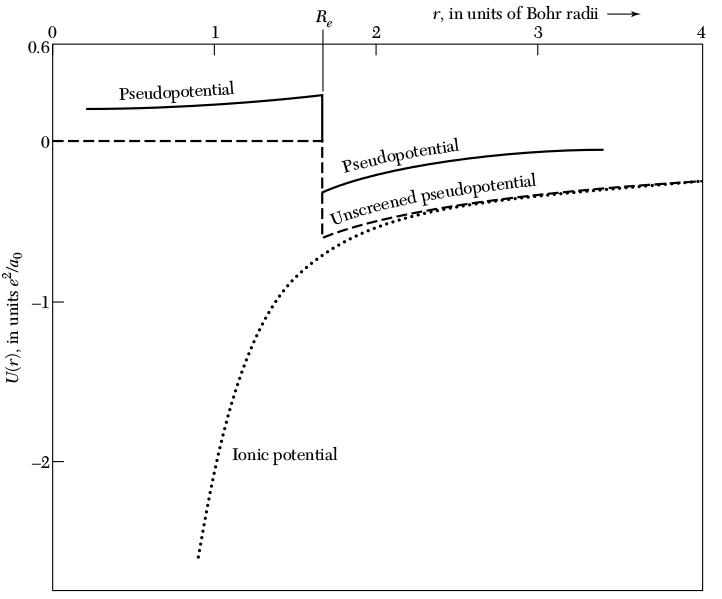
\includegraphics[height=1.60in,width=2.57in,viewport=0 0 980 600,clip]{Figures/Pseudo-model-empty_core.png}
\caption{\tiny \textrm{Pseudopotential for metallic sodium, based on the empty core model and screened by the Thomas-Fermi dielectric function.}}%(与文献\cite{EPJB33-47_2003}图1对比)
\label{Pseudo_model-empty_core}
\end{figure}
}

\frame
{
	\frametitle{传统赝势的构造}
\begin{figure}[h!]
\centering
\vspace*{-0.10in}
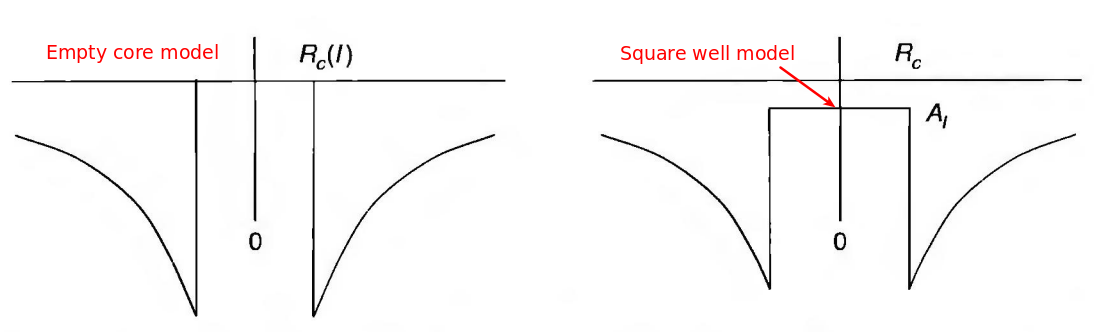
\includegraphics[height=1.30in,width=4.17in,viewport=0 0 1150 350,clip]{Figures/Pseudo-model.png}
\caption{\tiny \textrm{Left:``Empty core'' model potential of Ashcroft in which the potential is zero inside radius $R_c(l)$ which is different for each $l$. Right: Square well model potential with value $A_l$ inside a cut-off radius $R_c$, proposed by Abarenkov and Heine and fit to atomic data by Animalu and Heine. The fact that the potential are weak, zero, or even positive inside cut-off radius $R_c$ is an illustration of the ``cancellation theorem''.}}%(与文献\cite{EPJB33-47_2003}图1对比)
\label{Pseudo-model}
\end{figure}
}

\frame
{
	\frametitle{第一原理赝势}
		由第一原理求解出全电子波函数(径向部分)$P_{n,l}(r)$
			\begin{displaymath}
				\bigg[-\dfrac12\dfrac{\mathrm{d}^2}{\mathrm{d}r^2}\textcolor{blue}{+\dfrac{l(l+1)}{2r^2}}+V(\rho,r)\bigg]P_{n,l}(r)=\varepsilon_{n,l}P_{n,l}(r)
			\end{displaymath}
			这里$V(\rho,r)$是自洽单电子势
			$$V(\rho,r)=-\frac{Z}r+V_{\mathrm H}(\rho,r)+V_{XC}^{\mathrm{LDA}}(\rho(r))$$
			$V_{\mathrm H}(\rho,r)$是\textrm{Hartree}势,$V_{XC}^{\mathrm{LDA}}(\rho(r))$是交换-相关势

			由此构造赝波函数$P_l^{\mathrm{PS}}(r)$,满足
			$$P_l^{\mathrm{PS}}(r)=P_l^{\mathrm{AE}}(r),\quad r>r_{cl}$$
			进而构造赝势$V_{\mathrm{src},l}^{\mathrm{PP}}(r)$
			$$V_{\mathrm{src},l}^{\mathrm{PP}}(r)=\textcolor{red}{\varepsilon_l}\textcolor{magenta}{-\dfrac{l(l+2)}{2r^2}}+\dfrac{1}{2P_l^{\mathrm{PS}}(r)}\dfrac{\mathrm{d}^2}{\mathrm{d}r^2}P_l^{\mathrm{AE}}(r),\quad r>r_{cl}$$
}

\frame
{
	\frametitle{模守恒\textrm{(Norm-conserving)}条件}
%	构造赝势确定参数的边界(构造条件)
	\begin{enumerate}
		\item 价电子赝波函数的能量本征值与对应全电子波函数能量本征值相等:~$\varepsilon_l^{\mathrm{PP}}=\varepsilon_l^{\mathrm{AE}}$
		\item 价电子赝波函数与真实电子波函数的径向部分在截断半径$r_{c,l}$外相同:~$\psi_l^{\mathrm{PP}}(r)=\psi_l^{\mathrm{AE}}(r),\quad r>r_{cl}$
		\item 价电子赝波函数与真实电子波函数的对数导数在截断半径$r_{c,l}$处相等:~$D_l^{\mathrm{PP}}(r)=D_l^{\mathrm{AE}}(r),\quad r\geqslant r_{cl}$(\textcolor{blue}{可移植性基础})\\
			这里\textcolor{red}{$D_l(\varepsilon,r)=r\frac{\psi_l^{\prime}(\varepsilon,r)}{\psi_l(\varepsilon,r)}=r\dfrac{\mathrm{d}}{\mathrm{d}r}\ln\psi_l(\varepsilon,r)$}
		\item 价电子赝波函数与真实电子波函数在截断半径$r_{c,l}$内的积分电荷相等(\textcolor{red}{模守恒条件})
			$$Q_l=\int_0^{r_{cl}}\mathrm{d}rr^2|\psi_l^{\mathrm{PP}}(r)|^2=\int_0^{r_{cl}}\mathrm{d}rr^2|\psi_l^{\mathrm{AE}}(r)|^2$$
		\item \textcolor{magenta}{价电子赝波函数与真实电子波函数的对数导数一阶能量导数$\mathrm{d}D_l(\varepsilon,r)/\mathrm{d}\varepsilon$在截断半径$r_{c,l}$处及以外相等(强化可移植性)}
	\end{enumerate}
}

\frame
{
	\frametitle{模守恒\textrm{(Norm-conserving)}条件}
\begin{figure}[h!]
\centering
\vspace*{-0.10in}
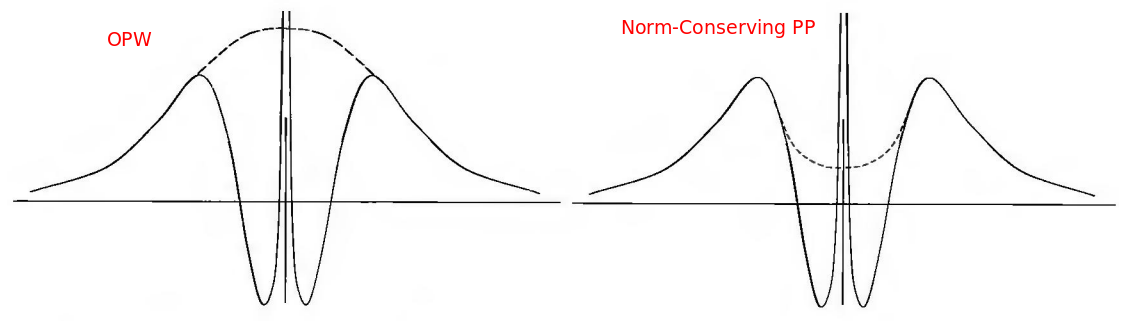
\includegraphics[height=1.30in,width=4.17in,viewport=0 0 1150 350,clip]{Figures/Pseudo-OPW_NCPP.png}
\caption{\tiny \textrm{Schematic example of a valence function that has the character of a $3s$ orbital near the nucleus and two examples of smooth functions (dashed lines) that equal the full wave-function outside the core region. Left: the smooth part of the valence function defined by OPW-like equation; Right: a smooth pseudo-function that satisfies the norm-conservation condition.}}%(与文献\cite{EPJB33-47_2003}图1对比)
\label{Pseudo-OPW_NCPP}
\end{figure}
}

\subsection{可分离赝势与\rm{Ghost~band}}
\frame
{
\frametitle{角动量$l$相关赝势}
由原子赝波函数(径向部分)构造赝势类似于求解类\textrm{H}原子波函数

赝原子波函数的径向部分是轨道角动量依赖的
\begin{displaymath}
	\psi_l^{\mathrm{PS}}(r)=r\phi_l^{\mathrm{PS}}(r)
\end{displaymath}
因此得到赝势函数(径向部分)$V_l(r)$也是角动量依赖的

为提高赝势的可移植性,减少构造赝势对环境的依赖,需要对其进行``去屏蔽''
\begin{displaymath}
	V_l(r)\equiv V_{l,src}^{\mathrm{PP}}-V_{\mathrm{Hartree}}^{\mathrm{PP}}(r)+V_{\mathrm{XC}^{PP}}(r)
\end{displaymath}

实际应用时习惯将赝势(径向部分)分解为\textcolor{blue}{局域部分(与角动量$l$无关)}和\textcolor{red}{非局域部分}
\begin{displaymath}
	V_l(r)=V_{\mathrm{local}}(r)+\delta V_l(\vec r)
\end{displaymath}
\textcolor{magenta}{考虑角度部分后,角动量$l$相关的赝势$\delta V_l$将是半局域
\begin{displaymath}
	V_{\mathrm{SL}}=V_{\mathrm{local}}(r)+\sum_{lm}|Y_{lm}\rangle\delta V_l\langle Y_{lm}|
\end{displaymath}}
}

\frame
{
	\frametitle{角动量$l$相关赝势}
	赝势是在原子(或离子)条件下构造的,它依赖于能量$\varepsilon_l$的选择
	\begin{displaymath}
		V_l(r,\varepsilon_l)=V_{\mathrm{local}}(r)+\delta V_l(r,\varepsilon_l)
	\end{displaymath}
	在原子、分子构型下,一般取无穷远为势能零点:~\textcolor{blue}{$\varepsilon<0$}
	\begin{itemize}
		\item \textcolor{purple}{在无限扩展的周期体系中,势能平均值(能量的参考零点)是无法确定的}\\
			构造第一原理赝势时,需要考虑参数$\varepsilon_l$的值无法唯一确定带来的影响
		\item 构造\textrm{PK}型赝势时,能量参数为$\varepsilon_v-\varepsilon_c$:\\
			能量差不依赖周期体系势能的平移常数,不存在上述问题
	\end{itemize}
}

\frame
{
	\frametitle{角动量$l$相关赝势计算的困难与克服}
	半局域型赝势在用平面波展开时,需要计算大量($\vec k$和$\vec k^{\prime}$都相关)的积分项
	\begin{displaymath}
		\int j_l(k\cdot r)V_l(r)j_l(k^{\prime}\cdot r)r^2\mathrm{d}rP_l(\cos\theta_{kk^{\prime}})
	\end{displaymath}
	这里$j_l$是球\textrm{Bessel}函数\\
	$P_l(\cos\theta_{kk^{\prime}})$是矢量$\vec k$和$\vec k^{\prime}$夹角的\textrm{Legendre}多项式函数
\vskip 8pt
\textrm{Kleinman-Bylander}等注意到:~如果角动量$l$相关的半局域型赝势可写成类似\textrm{PK}型赝势的形式,则平面波展开可写成
\begin{displaymath}
	\int j_l(k\cdot r)\textcolor{blue}{\varphi_l^c(r)}(r)r^2\mathrm{d}r\int j_l(k^{\prime}\cdot r^{\prime})\textcolor{blue}{\varphi_l^c(r^{\prime})}r^{\prime2}\mathrm{d}r^{\prime}P_l(\cos\theta_{kk^{\prime}})
\end{displaymath}
显然,大量积分将以乘积形式出现,因此需要独立计算的积分(仅与$\vec k$相关)数量将大大减少
}

\frame
{
	\frametitle{非局域赝势的变量分离}
	\textrm{Kleinman-Bylander}仿照\textrm{PK}型赝势的特点,提出了非局域赝势的变量分离方案\footnote{\fontsize{7.0pt}{4.2pt}\selectfont{即$\delta V(\vec r,\vec r^{\prime})$可以写成$\delta V(\vec r,\vec r^{\prime})=\sum_{i}f_i(\vec r)g_i(\vec r^{\prime})$的形式}}:~\\
%	引入分离算符$\delta V^{\mathrm{NL}}$满足
	如果选择适当的局域函数$V_{\mathrm{local}}^{\mathrm{PP}}(r)$,赝势将可分解为局域部分与非局域部分之和(这种分解称为\textrm{factored pseudo-potential})
	$$\hat V_{\mathrm{NL}}^{\mathrm{PP}}(r)=V_{\mathrm{local}}^{\mathrm{PP}}(r)+\sum_{lm}\dfrac{|\psi_{lm}^{\mathrm{PS}}\delta V_l\rangle\langle\delta V_l\psi_{lm}^{\mathrm{PS}}|}{\langle\psi_{lm}^{\mathrm{PS}}|\delta V_l|\psi_{lm}^{\mathrm{PS}}\rangle}$$ 
	\textcolor{magenta}{这是将$\delta V_l$表示到$\psi_{lm}^{\mathrm{PS}}$构成的空间中,$\langle\delta V_l(r)\psi_{lm}^{\mathrm{PP}}|$是投影子}
	
	\begin{displaymath}
		\langle\delta V_l\psi_{lm}^{\mathrm{PS}}|\psi\rangle=\int\mathrm{d}\vec r\delta V_l(r)\psi_{lm}^{\mathrm{PS}}(\vec r)\psi(\vec r)
	\end{displaymath}
	\textcolor{blue}{投影函数局域在截断半径内},该区域内$\delta V_l$有非零值
\begin{itemize}
	\item \textcolor{blue}{投影函数的存在,保证了即使非束缚态也可以作为赝波函数}
\end{itemize}
}

\frame
{
	\frametitle{非局域赝势的变量分离}
	应用投影函数,非局域赝势矩阵元的计算也变得更方便
	\begin{displaymath}
		\langle\psi_i|\delta V_{\mathrm{NL}}|\psi_j\rangle=\sum_{lm}\langle\psi_i|\psi_{lm}^{\mathrm{PS}}\delta V_l\rangle\frac1{\langle\psi_{lm}^{\mathrm{PS}}|\delta V_l|\psi_{lm}^{\mathrm{PS}}\rangle}\langle\delta V_l\psi_{lm}^{\mathrm{PS}}|\psi_j\rangle
	\end{displaymath}
	更一般地,如果允许赝势局域部分$V_{\mathrm{local}}^{\mathrm{PP}}(r)$为任意函数,则可定义辅助函数
	$$\chi_{lm}^{\mathrm{PS}}(\vec r)=\bigg\{\varepsilon_l-\bigg[-\dfrac12\nabla^2+V_{\mathrm{local}}^{\mathrm{PP}}(\vec r)\bigg]\bigg\}\psi_{lm}^{\mathrm{PS}}(\vec r)$$
	于是赝势的非局域部分可表示为
	$$\delta V_{\mathrm{NL}}=\sum_{lm}\dfrac{|\chi_{lm}^{\mathrm{PS}}\rangle\langle\chi_{lm}^{\mathrm{PS}}|}{\langle\chi_{lm}^{\mathrm{PS}}|\psi_{lm}^{\mathrm{PS}}\rangle}$$

但是$V_{\mathrm{local}}^{\mathrm{PP}}(r)$选择的随意性,将增加计算结果出现\textrm{Ghost~band}的风险
}

\frame
{
	\frametitle{\textrm{Ghost~band}的表现}
	\fontsize{9.2pt}{4.2pt}\selectfont{只有价电子的赝波函数与芯电子波函数完全正交,能带计算中才能确保芯层与价层电子的完全分离。但实际计算时,该正交条件很难严格保证,因此一旦赝波函数严重偏离正交条件,计算的能带中会在本不存在能带的区域出现电子结构分布(称为\textrm{Ghost~band}),这部分电子结构源自构造赝波函数的能量参数$\varepsilon_l$与芯层电子能量差别太大,无法保持与芯层电荷严格正交引起的}
\begin{figure}[h!]
\centering
\vspace*{-0.10in}
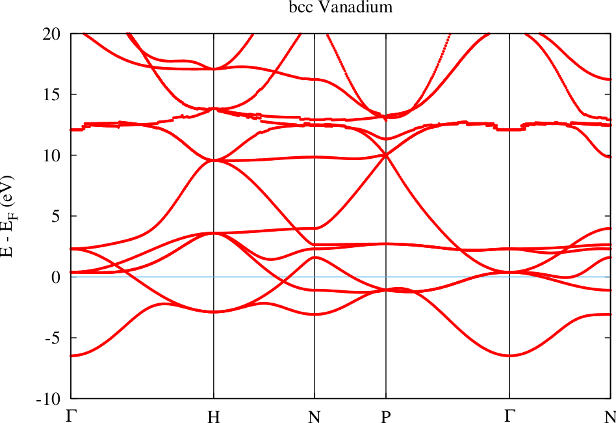
\includegraphics[height=1.50in,width=1.98in,viewport=0 0 450 320,clip]{Figures/Ghostband-Vanadium-1.png}
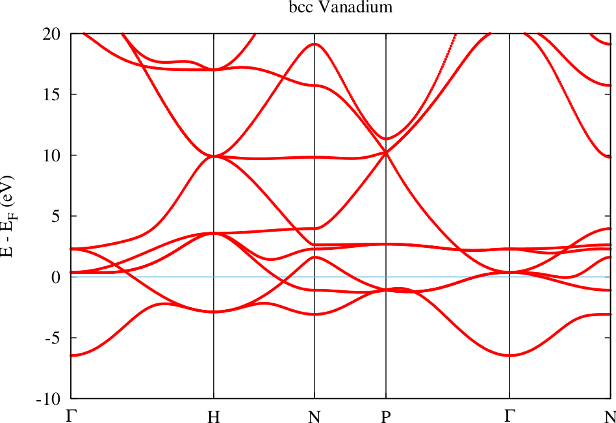
\includegraphics[height=1.50in,width=1.98in,viewport=0 0 450 320,clip]{Figures/Ghostband-Vanadium-4.png}
\caption{\fontsize{7.2pt}{4.2pt}\selectfont{\textrm{The band structure of bcc Vanadium. %In the calculation, all electrons up to the 3p states were treated as core electrons, all other electrons as valence electrons. 
\\Left:~Between 10 and 15 eV above the Fermi energy a strange band with nearly no dispersion can be observed. The vanishing dispersion of the band is a typical property of ghost bands.}}}%(与文献\cite{EPJB33-47_2003}图1对比)
\label{Ghost-band}
\end{figure}
}

\frame
{
	\frametitle{\textrm{Ghost~band}的根源}
	可分离赝势方法中
	\begin{displaymath}
		\hat{\mathbf{H}}=-\dfrac12\nabla^2+V_{\mathrm{local}}(r)+\delta\hat{V}_{\mathrm{NL}}
	\end{displaymath}
	赝波函数$\psi_{lm}^{\mathrm{PP}}(r)$是方程
	\begin{displaymath}
		\hat{\mathbf{H}}\psi_{lm}^{\mathrm{PP}}(r)=\varepsilon_l\psi_{lm}^{\mathrm{PP}}(r)
	\end{displaymath}
	的解。
\vskip 15pt
	因为$V_{\mathrm{local}}(r)$可随意选择,因此赝波函数$\psi_{lm}^{\mathrm{PP}}(r)$和能量$\varepsilon_l$不再要求与束缚态波函数相对应,将导致\textrm{Ghost~band}的出现
}

\frame
{
	\frametitle{\textrm{Ghost~band}根源的数学说明$^{\ast}$}
	{\fontsize{7.2pt}{5.2pt}\selectfont{对于半局域势,求解能量$\varepsilon$对应的径向波函数$u_l(r,\varepsilon)$的方程\textcolor{blue}{是一个常微分方程}
		\begin{displaymath}
			-\dfrac12\dfrac{\mathrm{d}^2u_l}{\mathrm{d}r^2}+\overline{V}_l^{\mathrm{loc}}(r)u_l(r,\varepsilon)+\Delta V_l^{\mathrm{SL}}(r)u_l(r,\varepsilon)-\varepsilon u_l(r,\varepsilon)=0
		\end{displaymath}
		而对于可分离赝势(如\textrm{KB}势),方程则为\textcolor{blue}{积分-微分方程}
		\begin{displaymath}
			-\dfrac12\dfrac{\mathrm{d}^2u_l}{\mathrm{d}r^2}+\overline{V}_l^{\mathrm{loc}}(r)u_l(r,\varepsilon)+\int\Delta V_l(r,r^{\prime})u_l(r^{\prime},\varepsilon)\mathrm{d}r^{\prime}-\varepsilon u_l(r,\varepsilon)=0
		\end{displaymath}
		将可分离赝势代入可有
		\begin{displaymath}
			-\dfrac12\dfrac{\mathrm{d}^2u_l}{\mathrm{d}r^2}+\overline{V}_l^{\mathrm{loc}}(r)u_l(r,\varepsilon)+f_l(r)\int g_l(r^{\prime})u_l(r^{\prime},\varepsilon)\mathrm{d}r^{\prime}-\varepsilon u_l(r,\varepsilon)=0
		\end{displaymath}
		\begin{itemize}
			\item \textcolor{blue}{常微分方程解的结构服从\textrm{Wronskian}定理的推论:~本征态能量$\varepsilon_0,\varepsilon_1,\cdots,\varepsilon_n$按升序排列时,对应的本征态波函数(径向)的节点数依次递增}
			\item \textcolor{red}{积分-微分方程解的结构不要求满足该结论:~波函数的节点数与能量本征态不再有对应的升序关系}
		\end{itemize}
		由于积分项的存在,传统的常微分方程求解算法(如\textrm{Runger-Kutta}法等)无法直接用于该积分-微分方程,必须另图别策
	}}
}

\frame
{
	\frametitle{\textrm{Ghost~band}根源的数学说明$^{\ast}$}
		{\fontsize{7.2pt}{5.2pt}\selectfont{
		基本思想:~类似积分方程求解的\textrm{Fredholm}方法
		\begin{itemize}
			\item 先将微分方程中的\textcolor{magenta}{积分项近似为常数因子},\textcolor{blue}{求解非齐次常微分方程}
			\item 对含有波函数的积分,应用闭路积分公式\textrm{(closure formula)}计算
		\end{itemize}}}
		{\fontsize{5.2pt}{5.2pt}\selectfont{具体求解流程
		\begin{enumerate}
			\item 采用通用方法分别求解\\\textcolor{blue}{齐次微分方程}
				\begin{displaymath}
					-\dfrac12\dfrac{\mathrm{d}^2W_l}{\mathrm{d}r^2}+\overline{V}_l^{\mathrm{loc}}(r)W_l(r,\varepsilon)-\varepsilon W_l(r,\varepsilon)=0
				\end{displaymath}
				的通解和\\\textcolor{magenta}{不含积分项的}\textcolor{blue}{非齐次微分方程}
				\begin{displaymath}
					-\dfrac12\dfrac{\mathrm{d}^2X_l}{\mathrm{d}r^2}+\overline{V}_l^{\mathrm{loc}}(r)X_l(r,\varepsilon)-\varepsilon X_l(r,\varepsilon)=f_l(r)
				\end{displaymath}
				的一个特解
			\item 构造积分
				\begin{displaymath}
					\begin{aligned}
					\tilde {W}(\varepsilon)=&\int g_l(r)W(r,\varepsilon)\mathrm{d}r\\
					\tilde {X}(\varepsilon)=&1+\int g_l(r)X(r,\varepsilon)\mathrm{d}r
					\end{aligned}
				\end{displaymath}
			\item 由此得到积分-微分方程的解
				\begin{displaymath}
					u(r,\varepsilon)=K[W(r,\varepsilon)\tilde{X}(\varepsilon)-X(r,\varepsilon)\tilde{W}(\varepsilon)]
				\end{displaymath}
		这里$K$是归一化因子	
		\end{enumerate}
	}}
}

\frame
{
	\frametitle{\textrm{Ghost~band}的克服}
	{\fontsize{7.2pt}{5.2pt}\selectfont{根据微分方程理论
	\begin{displaymath}
		\hat{\mathbf{H}}\psi_{lm}^{\mathrm{PP}}(r)=\varepsilon_l\psi_{lm}^{\mathrm{PP}}(r)
	\end{displaymath}
	的解$\psi_{lm}^{\mathrm{PP}}(r)$可表示为(只考虑径向部分)
	\begin{displaymath}
		\psi_{l}^{\mathrm{PP}}(r)=u_l^0(r)+\sum_ic_iu_l^i(r)
	\end{displaymath}
这里$u_l^0(r)$和$u_l^i(r)$分别是
齐次微分方程
	\begin{displaymath}
		\bigg(-\dfrac12\nabla^2+V_{\mathrm{local}}-\varepsilon_l^0\bigg)u_{l}^0(r)=0
	\end{displaymath}
和非齐次微分方程
	\begin{displaymath}
		\bigg(-\dfrac12\nabla^2+V_{\mathrm{local}}-\varepsilon_l^j\bigg)u_{l}^j(r)=\chi_{l}^j(r)
	\end{displaymath}
的解

引入多个能量参数$\varepsilon_l^i$,通过优化控制参数$c_i$,可以得到理想的局域势函数$V_{\mathrm{local}}(r)$
}}
}

\frame
{
	\frametitle{广义模守恒条件}
	为提高模守恒赝势的可移植性\footnote{\tiny{换言之,提升赝波函数能适应的能量变分空间}},\textrm{Vanderbilt}和\textrm{Bl\"ochl}分别建议:\\
	在构造可分离赝势时,\textcolor{blue}{引入额外的参考能量$\varepsilon_l$,并要求对每个角动量量子数$l$,所有能量参数$\varepsilon_l$构造的赝波函数$\phi_i^{\mathrm{ps}}$及其辅助函数$\chi_i$都满足
	\begin{displaymath}
		|\chi_i\rangle=-(\mathbf{T}+V_{\mathrm{loc}}-\varepsilon)|\phi_i^{\mathrm{ps}}\rangle
	\end{displaymath}}
	{\fontsize{7.2pt}{5.2pt}\selectfont{这里$i$表示量子数$l$,$m$和能量参数$\varepsilon$,即$i=(lm,\varepsilon)$}}
	\vskip 5pt
	由此出发,可构造出一组与赝波函数$\phi_i^{\mathrm{ps}}$垂直的函数$\beta_i$:~
{\fontsize{7.2pt}{5.2pt}\selectfont{
	\begin{itemize}
		\item 构造矩阵$\mathbf{B}$,其矩阵元$B_{ij}$满足
			\begin{displaymath}
				B_{ij}= \langle\phi_j^{\mathrm{ps}}|\chi_i\rangle
			\end{displaymath}
		\item 由矩阵$\mathbf{B}$和$\chi$得到函数$\beta_i$
			\begin{displaymath}
				|\beta_i\rangle=\sum_j(\mathbf{B}^{-1})_{ij}|\chi_j\rangle
			\end{displaymath}
		\item 由此得到的$\beta$与赝波函数$\phi_i^{\mathrm{ps}}$满足正交条件
	\begin{displaymath}
		\langle\beta_i|\phi_j^{\mathrm{ps}}\rangle=\delta_{ij}
	\end{displaymath}
	\end{itemize}}}
}

\frame
{
	\frametitle{广义模守恒条件}
	因此可分离赝势的非局域部分表示为
	\textcolor{blue}{\begin{displaymath}
		V_{\mathrm{NL}}=\sum_i|\chi_i\rangle\langle\beta_i|=\sum_{ij}B_{ij}|\beta_j\rangle\langle\beta_i|
	\end{displaymath}}
	{\fontsize{7.2pt}{5.2pt}\selectfont{不难看出,如果赝波函数满足广义模守恒条件
	\begin{displaymath}
		Q_{ij}=\langle\phi_j^{\mathrm{AE}}|\phi_i^{\mathrm{AE}}\rangle-\langle\phi_j^{\mathrm{PS}}|\phi_i^{\mathrm{PS}}\rangle = 0
	\end{displaymath}
	亦即
	\begin{displaymath}
		Q_{l\varepsilon,l\varepsilon^{\prime}}=\int_0^{R_c}\bigg(\phi_{l\varepsilon}^{\mathrm{AE}}(r)\phi_{l\epsilon^{\prime}}^{\mathrm{AE}}(r)-\phi_{l\varepsilon}^{\mathrm{PS}}(r)\phi_{l\varepsilon^{\prime}}^{\mathrm{PS}}(r)\bigg)\mathrm{d}r=0
	\end{displaymath}
	将大大提高赝势的可移植性。
	\vskip 5pt
	但实际上,广义模守恒条件看似简单,当能量参数$\varepsilon\neq\varepsilon^{\prime}$,要满足这个条件
	$$Q_{l\varepsilon,l\varepsilon^{\prime}}=0$$
	并非易事;~而一旦模守恒条件被破坏,矩阵$\mathbf{B}$(相应地,赝势的非局域部分$V_{\mathrm{NL}}$)就是非\textrm{Hermitian}}}
}

\frame
{
\frametitle{超软赝势}
\begin{itemize}
\setlength{\itemsep}{5pt}
	\item 赝势构造的模守恒条件
%		\begin{displaymath}
%			\int_0^{r_c}\mathrm{d}\vec r\varphi^{\ast PS}(\vec r)\varphi^{PS}(\vec r)=\int_0^{r_c}\mathrm{d}\vec r\varphi^{\ast}(\vec r)\varphi(\vec r)
%		\end{displaymath}
	很好地解决了赝势可移植性问题,但对$1s$、$2p$、$3d$等轨道,模守恒方案构造的赝势过于“硬”,所需平面波基组依然非常大
	\item 超软\textrm{(Ultra-soft)}赝势,解除模守恒条件,实现对第一、第二周期元素的高效计算
\end{itemize}
\begin{figure}[h!]
\vspace*{-0.10in}
\centering
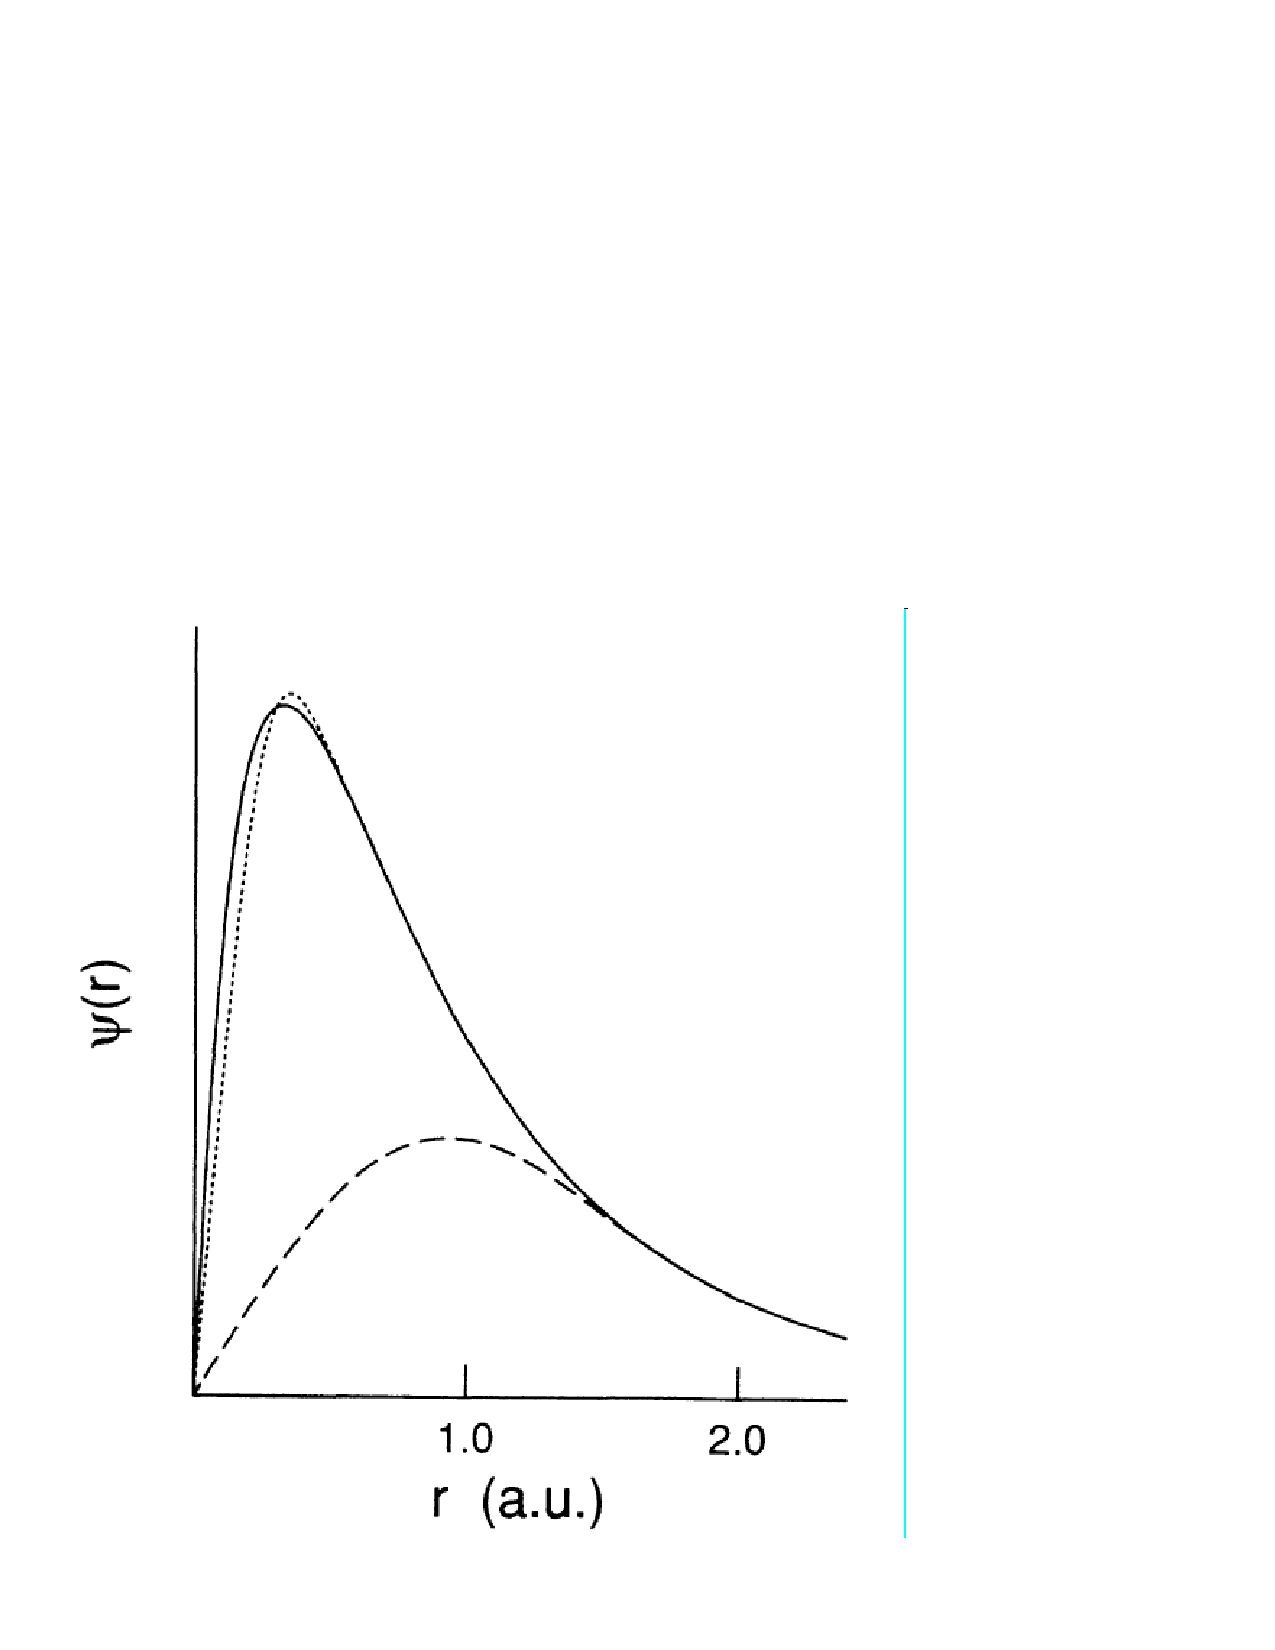
\includegraphics[height=1.35in,width=1.40in,viewport=30 55 415 500,clip]{Figures/Norm-US-wave.pdf}
\caption{\tiny \textrm{Oxygen 2} \textit{p} \textrm{radical wave function (solid), NC-pseudo-wave (dotted) and US-pseudo-wave (dashed).}}%(与文献\cite{EPJB33-47_2003}图1对比)
\label{Norm-US-wave}
\end{figure}
}

\frame
{
	\frametitle{从模守恒赝势到超软赝势}
	为提高模守恒赝势的可移植性\footnote{\tiny{换言之,提升赝波函数能适应的能量变分空间}},\textrm{Vanderbilt}和\textrm{Bl\"ochl}分别建议:\\
	在构造可分离赝势时,\textcolor{blue}{引入额外的参考能量$\varepsilon_l$,并要求对每个角动量量子数$l$,所有能量参数$\varepsilon_l$构造的赝波函数$\phi_i^{\mathrm{ps}}$及其辅助函数$\chi_i$都满足
	\begin{displaymath}
		|\chi_i\rangle=-(\mathbf{T}+V_{\mathrm{loc}}-\varepsilon)|\phi_i^{\mathrm{ps}}\rangle
	\end{displaymath}}
	{\fontsize{7.2pt}{5.2pt}\selectfont{这里$i$表示量子数$l$,$m$和能量参数$\varepsilon$,即$i=(lm,\varepsilon)$}}
	\vskip 5pt
	由此出发,可构造出一组与赝波函数$\phi_i^{\mathrm{ps}}$垂直的函数$\beta_i$:~
{\fontsize{7.2pt}{5.2pt}\selectfont{
	\begin{itemize}
		\item 构造矩阵$\mathbf{B}$,其矩阵元$B_{ij}$满足
			\begin{displaymath}
				B_{ij}= \langle\phi_j^{\mathrm{ps}}|\chi_i\rangle
			\end{displaymath}
		\item 由矩阵$\mathbf{B}$和$\chi$得到函数$\beta_i$
			\begin{displaymath}
				|\beta_i\rangle=\sum_j(\mathbf{B}^{-1})_{ij}|\chi_j\rangle
			\end{displaymath}
		\item 由此得到的$\beta$与赝波函数$\phi_i^{\mathrm{ps}}$满足正交条件
	\begin{displaymath}
		\langle\beta_i|\phi_j^{\mathrm{ps}}\rangle=\delta_{ij}
	\end{displaymath}
	\end{itemize}}}
}

\frame
{
	\frametitle{从模守恒赝势到超软赝势}
	因此可分离赝势的非局域部分表示为
	\textcolor{blue}{\begin{displaymath}
		V_{\mathrm{NL}}=\sum_i|\chi_i\rangle\langle\beta_i|=\sum_{ij}B_{ij}|\beta_j\rangle\langle\beta_i|
	\end{displaymath}}
	{\fontsize{7.2pt}{5.2pt}\selectfont{不难看出,如果赝波函数满足广义模守恒条件
	\begin{displaymath}
		Q_{ij}=\langle\phi_j^{\mathrm{AE}}|\phi_i^{\mathrm{AE}}\rangle-\langle\phi_j^{\mathrm{PS}}|\phi_i^{\mathrm{PS}}\rangle = 0
	\end{displaymath}
	亦即
	\begin{displaymath}
		Q_{l\varepsilon,l\varepsilon^{\prime}}=\int_0^{R_c}\bigg(\phi_{l\varepsilon}^{\mathrm{AE}}(r)\phi_{l\epsilon^{\prime}}^{\mathrm{AE}}(r)-\phi_{l\varepsilon}^{\mathrm{PS}}(r)\phi_{l\varepsilon^{\prime}}^{\mathrm{PS}}(r)\bigg)\mathrm{d}r=0
	\end{displaymath}
	将大大提高赝势的可移植性。
	\vskip 5pt
	但实际上,广义模守恒条件看似简单,当能量参数$\varepsilon\neq\varepsilon^{\prime}$,要满足这个条件
	$$Q_{l\varepsilon,l\varepsilon^{\prime}}=0$$
	并非易事;~而一旦模守恒条件被破坏,矩阵$\mathbf{B}$(相应地,赝势的非局域部分$V_{\mathrm{NL}}$)就是非\textrm{Hermitian}}}
}

\frame
{
\frametitle{超软赝势的构造}
\textrm{Vanderbilt}建议构造赝波函数时放弃模守恒约束条件,只要求价电子赝波函数与真实电子波函数的径向部分在截断半径$r_{c,l}$外相同,由此得到的赝势显然非\textrm{Hermitian},但是通过构造\\\textcolor{blue}{\textrm{Hermitian}重叠算符}
\begin{displaymath}
	\mathbf{S}=\mathbf{1}+\sum_{i,j}Q_{ij}|\beta_j\rangle\langle\beta_i|
\end{displaymath}
以及\textcolor{blue}{\textrm{Hermitian}赝势算符}
\begin{displaymath}
	\tilde V^{\mathrm{NL}}=\sum_{i,j}\mathbf{D}_{i,j}|\beta_j\rangle\langle\beta_i|
\end{displaymath}
这里\textcolor{blue}{
\begin{displaymath}
	\mathbf{D}_{ij}=B_{ij}+\varepsilon_iQ_{ij}
\end{displaymath}}
模守恒约束下的标准本征值方程将变成广义本征值方程
\begin{displaymath}
	(T+V_{\mathrm{loc}}+\tilde V^{\mathrm{NL}}-\varepsilon\mathbf{S})|\phi\rangle=0
\end{displaymath}
}

\frame
{
\frametitle{超软赝势的特点}
\textrm{Vanderbilt}的超软赝势构造方案最大的优点是
\begin{itemize}
	\item \textcolor{purple}{解除模守恒约束}:~有助于增加赝波函数的截断半径,系统提高赝势的柔软程度
	\item \textcolor{purple}{引入多个参考能量$\varepsilon_l$}:~使得模守恒条件下只在特定参考能量$\varepsilon$处成立的对数导数连续条件,扩展到参考能量$\varepsilon_l$区间范围内,这大大提高了赝势的适用范围(可移植性)
\end{itemize}

相应的,超软赝势计算中,电子密度表达形式为
\begin{displaymath}
	n(r)=\sum_nf_n|\phi_n(r)|^2+\sum_{n,ij}f_n\langle\phi_n|\beta_j\rangle\langle\beta_i|\phi_n\rangle Q_{ij}(r)
\end{displaymath}
这里补偿电荷$Q_{ij}(r)$定义为
\begin{displaymath}
	Q_{ij}(r)=\phi_i^{\mathrm{AE}}(r)\phi_j^{\mathrm{AE}}(r)^{\ast}-\phi_i^{\mathrm{US}}(r)\phi_j^{\mathrm{US}}(r)^{\ast}
\end{displaymath}
}

\frame
{
\frametitle{补偿电荷与多极矩}
根据电动力学定理:\\\textcolor{blue}{如果球\textrm{S}内的电荷密度分布$\rho(\vec r)$,在球外某点$\vec r$产生的势是由电荷密度的多极矩确定}:
\begin{figure}[h!]
\vspace*{-15pt}
\centering
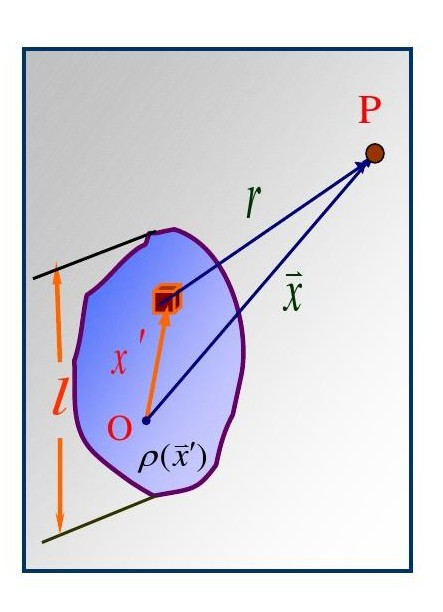
\includegraphics[height=1.25in,width=1.32in,viewport=1 22 507 575,clip]{Figures/potential_multipole.jpg}
%\caption{\tiny \textrm{From Muffin-tin Potential to Full Potential}}%(与文献\cite{EPJB33-47_2003}图1对比)
\label{Potential-multipole}
\end{figure}
\begin{displaymath}
	V(\vec r)=\sum_{l=0}^{\infty}\sum_{m=-l}^{l}\dfrac{4\pi}{2l+1}q_{lm}\dfrac{Y_{lm}(\hat{\vec r})}{r^{l+1}}
\end{displaymath}
其中多极矩$q_{lm}$由下式计算
\begin{displaymath}
	q_{lm}=\int_SY_{lm}^{\ast}(\hat{\vec r})r^l\rho(\vec r)\mathrm{d}^3r
\end{displaymath}
}

\subsection{\rm{VASP}中的\rm{PAW~}原子数据集}
\frame
{
%	\frametitle{\textrm{PAW}原子数据集}
	\frametitle{\textrm{PAW Augmentation}}
\begin{figure}[h!]
\centering
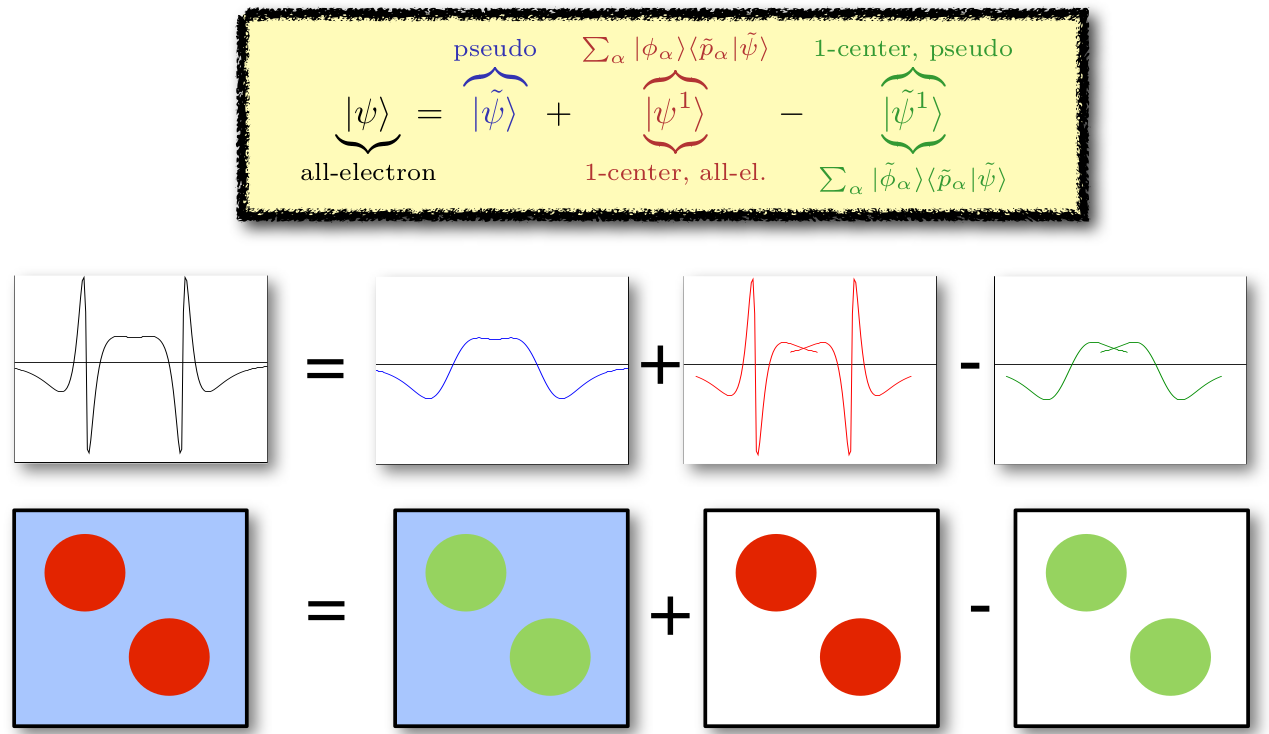
\includegraphics[height=2.3in,width=4.0in,viewport=0 0 1280 745,clip]{Figures/PAW-baseset.png}
\caption{\tiny \textrm{The Augmentation of PAW.}}%(与文献\cite{EPJB33-47_2003}图1对比)
\label{PAW_baseset}
\end{figure}
}

\frame
{
	\frametitle{\textrm{PAW}原子数据集}
	平滑赝原子分波函数
	\begin{displaymath}
		\tilde\phi_{i=Lk}(\vec r)=Y_L(\widehat{\vec r-\vec R})\tilde\phi_{lk}(|\vec r-\vec R|)
	\end{displaymath}
	根据\textrm{RRKJ}赝势构造,赝分波函数由球\textrm{Bessel}函数线性组合
	\begin{displaymath}
		\tilde\phi_{lk}(r)=\left\{
		\begin{aligned}
			&\sum_{i=1}^2\alpha_ij_l(q_ir)\quad &r<r_c^l\\
			&\phi_{lk}(r)\quad&r>r_c^l
		\end{aligned}
		\right.
	\end{displaymath}
	调节系数$\alpha_i$和$q_i$赝分波函数$\phi_{lk}(r)$在截断半径$r_c^l$处两阶连续可微
	投影子波函数$\tilde p_i$由\textrm{Gram-Schmidt}正交条件$\langle\tilde p_i|\tilde\phi_j\rangle=\delta_{ij}$确定
}

\frame
{
	\frametitle{\textrm{VASP}中的\textrm{PAW}原子数据集}
	\textcolor{blue}{构造原子局域赝势$\tilde v_{\mathrm {eff}}^a$}(\textcolor{red}{为防止\textrm{ghost band}}):\\在截断半径$r_{loc}$内的定义为
	$$\tilde v_{\mathrm {eff}}^a=A\dfrac{\sin(q_{loc}r)}r\quad r<r_{loc}$$
	其中$q_{loc}$和$A$要求局域赝势在截断半径$r_{loc}$处连续到一阶导数

	\textcolor{blue}{构造赝芯电荷密度$\tilde n_c$}:~在截断半径$r_{pc}$内的定义为
	$$\sum_{i=1,2}B_i\dfrac{\sin(q_ir)}r\quad r<r_{pc}$$
	调节系数$q_i$和$B_i$使得赝芯电荷密度$\tilde n_c(r)$在截断半径$r_{pc}$处的两阶导数连续

	局域离子赝势$v_H[\tilde n_{Zc}]$可由原子局域赝势去屏蔽得到
	$$v_H[\tilde n_{Zc}]=\tilde v_{\mathrm {eff}}^a-v_H[\tilde n_a^1+\hat n_a]-v_{\mathrm{XC}}[\tilde n_a^1+\hat n_a+\tilde n_c]$$
	在\textrm{VASP}的\textrm{POTCAR}生成过程中,各截断半径的确定条件
	$r_{rad}=\max({r_c^l})$,$r_{pc}\approx r_{rad}/1.2$,$r_{loc}<r_{rad}/1.2$
}

\frame
{
	\frametitle{\textrm{VASP}中的\textrm{PAW}原子数据集}
	在每个原子球内用球\textrm{Bessel}函数构造补偿电荷$g_l(r)$
	$$g_l(r)=\sum_{i=1}^2\alpha_i^lj_l(q_i^lr)$$
	调节系数$q_i^l$和$\alpha_i^l$使得补偿电荷$g_l(r)$在截断半径$r_{comp}$处的数值和前两阶导数值都是0,因此可以选择$q_i^l$使得多极矩
	$$\int_0^{r_{comp}}g_l(r)r^{l+2}\mathrm{d}r=1$$
	并且有
	$$\dfrac{\mathrm{d}}{\mathrm{d}r}j_l(q_i^lr)\bigg|_{r_{comp}}=0$$
	设置$\alpha_i^l$,因此$g_l(r_{comp})=0$,$r_{comp}=r_{rad}/1.3\sim r_{rad}/1.2$
}

\frame
{
	\frametitle{几种赝势方法的关系}
\begin{figure}[h!]
\centering
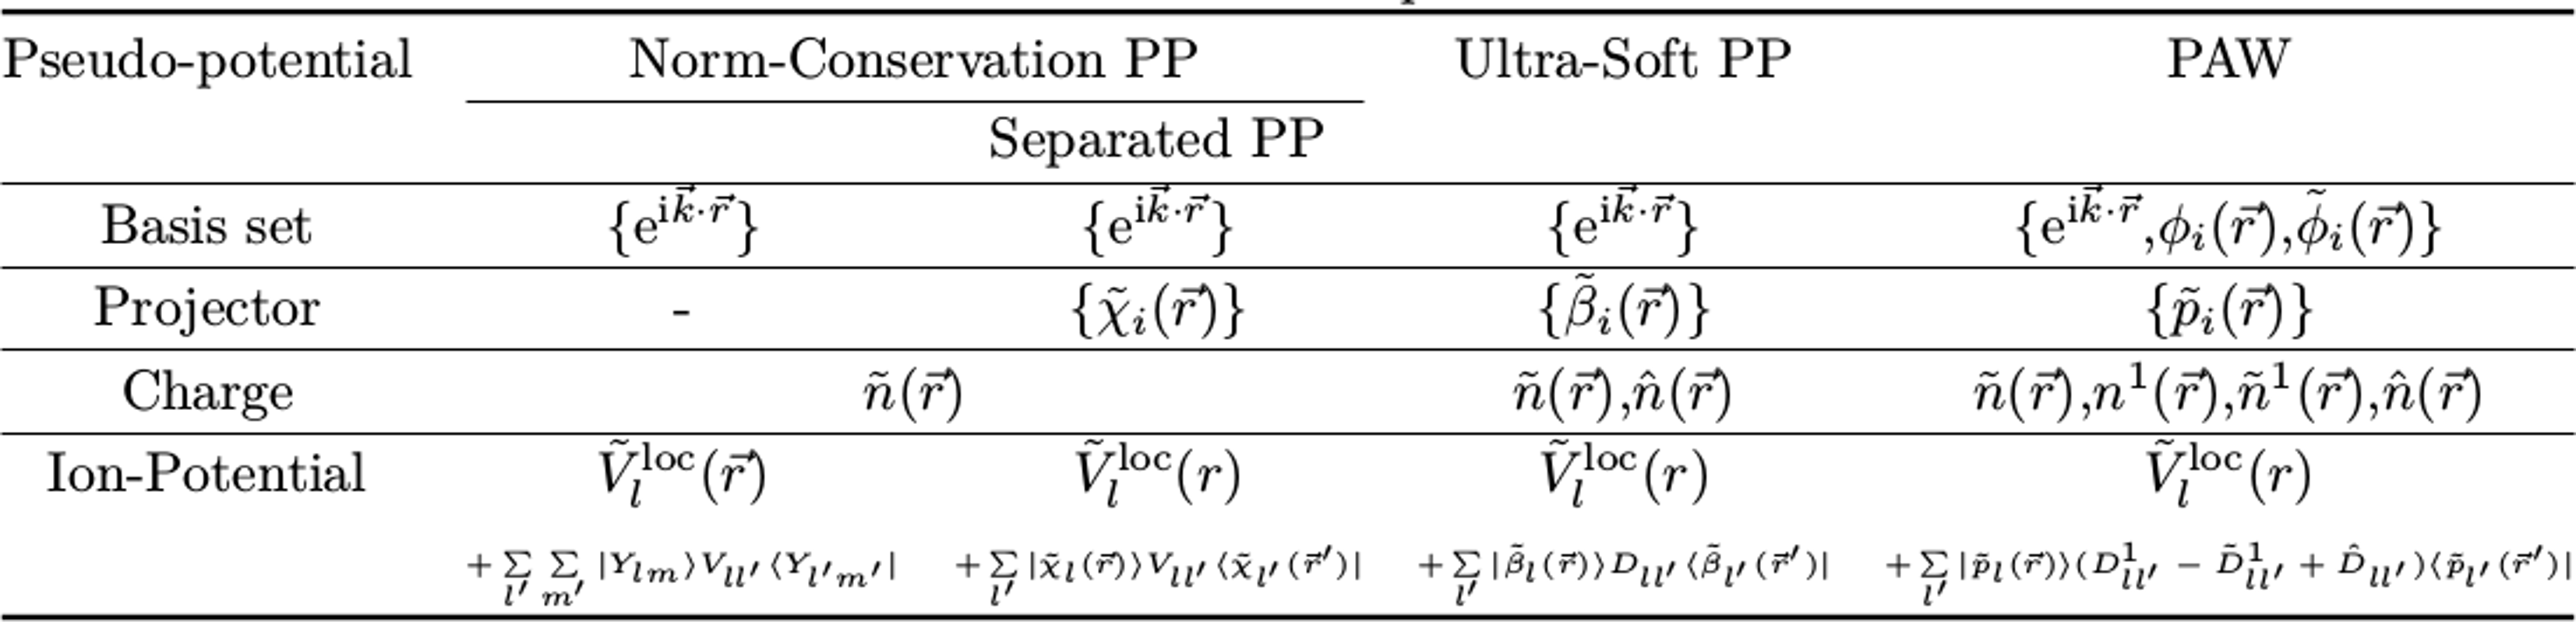
\includegraphics[height=1.0in,width=4.1in,clip]{Figures/Pseudo-Potential.png}
\caption{\tiny \textrm{The relation of Pseudo potential and PAW.}}%(与文献\cite{EPJB33-47_2003}图1对比)
\label{Pseudo_Potential_PAW}
\end{figure}
}

\section{\rm{AtomPAW}赝势\rm{Data set}的生成}
%\frame
%{
%	\frametitle{\textrm{AtomPAW}程序包简介}
%	\textrm{AtomPAW}程序包是由\textrm{Holzwarth}、\textrm{Tackett}和\textrm{Matthews}开发的\textrm{PAW}原子数据集生成程序,主要基于基于\textrm{Bl\"ochl}提出的原子数据集生成方案。
%
%	\textrm{AtomPAW}程序包产生的原子数据集,主要用于基于\textrm{PAW}方法的材料计算软件\textrm{PWPAW}和\textrm{ABINIT}。
%
%%\centering {\large \textrm{PP-PW}$\Longrightarrow$} \textbf{PP-PAW}$\Longleftrightarrow$\textbf{\textcolor{red}{FP-PAW}}{\large$\Longleftarrow$ \textrm{FP-LAPW}}
%%\begin{table}[!H]
%%\tabcolsep 5pt 
%%%\vspace*{-12pt}
%%%\caption{\textrm{The compare of directly diagonalization and $\vec k\cdot\vec p$ perturbation.}}
%%\vspace{5pt}
%%\label{Table-Compare_CaB6}
%%\begin{minipage}{\textwidth}
%%%\begin{center}
%%\centering
%%\def\temptablewidth{1.01\textwidth}
%%\rule{\temptablewidth}{1pt}
%%\begin{tabular*} {\temptablewidth}{@{\extracolsep{\fill}}cccc}
%%	& \textcolor{red}{基函数} & \textcolor{red}{\textrm{Coulomb}势}  &\textcolor{red}{总能量}  \\
%%	& \textrm{(PW}与球内分波\textrm{)} & \textrm{(}$\rho_I$与赝电荷$\hat n$\textrm{)}  &奇点排除  \\ \hline
%%	\textrm{LAPW}  &\textcolor{blue}{在球面上连续}       &\textcolor{blue}{简单叠加}        & \textcolor{blue}{需要考虑}\\
%%	\textrm{PAW}  &\textcolor{blue}{线性变换}:\textcolor{brown}{简单}        &\textcolor{blue}{线性变换}:\textcolor{brown}{复杂}    &\textcolor{blue}{需要考虑}\\
%%\end{tabular*}
%%\rule{\temptablewidth}{1pt}\\
%%%\end{center}
%%\end{minipage}
%%\end{table}
%}
%
%\frame
%{
%	\frametitle{\textrm{AtomPAW}的输入文件}
%	\textrm{AtomPAW}的输入文件主要包括
%	\begin{itemize}
%		\item 指定原子名称、核电荷数
%		\item 指定交换-相关泛函的形式和径向布点数
%		\item 指定原子核外电子的排布(电子组态)
%		\item 指定波函数展开所需分波最高角动量和各种半径\\$r_{paw}$、$r_{shape}$、$r_{vloc}$和$r_{core}$
%		\item 指定构造外加分波的能量参数$E_l$
%		\item 指定\textcolor{blue}{赝波函数、投影子函数(含正交化)和补偿电荷生成方案}
%		\item 指定\textcolor{blue}{局域势$v_{loc}(r)$生成方案}
%		\item 指定原子数据集输出方式
%	\end{itemize}
%}
%
%\frame
%{
%	\frametitle{\textrm{AtomPAW}的输出原子数据集文件}
%	\textrm{AtomPAW}的输出的原子数据集文件主要包括
%	\begin{itemize}
%		\item 计算中使用的控制参数
%		\item 原子价电子波函数$\phi_l(r_i)$
%		\item 价电子波函数的赝波函数$\tilde\phi_l(r_i)$
%		\item 投影子函数$\tilde p_l(r_i)$
%		\item 原子核附近真实价电荷密度$n^1(r_i)$
%		\item 赝电荷密度$\tilde n^1(r_i)$
%		\item 补充电荷密度$\hat n(r_i)$
%		\item 局域势$v_{loc}(r)$
%	\end{itemize}
%}

\frame
{
	\frametitle{\textrm{AtomPAW}程序的赝势构造}
	求解原子的价层的全电子分波函数
	{\fontsize{9.0pt}{5.2pt}\selectfont$$\hspace*{-17pt}\bigg(-\dfrac{\hbar^2}{2m}\nabla^2-\dfrac{Ze^2}r+e^2\int\mathrm{d}^3r^{\prime}\dfrac{n_{core}(r^{\prime})+n(r^{\prime})}{|r-r^{\prime}|}+\mu_{XC}[n_{core}(r)+n(r)]\bigg)|\phi_i\rangle=\epsilon_i|\phi_i\rangle$$}
	全电子分波电荷密度
	$$n(r)=\sum_{n,l}c_{n,l}\dfrac{|\phi_{n,l}(r)|^2}{4\pi r^2}$$
}

\frame
{
	\frametitle{\textrm{AtomPAW}程序的赝势构造}
	有效赝势的构造方案
	\begin{itemize}
		\item \textrm{Troullier-Martin NC} 方案 \\
	首先通过指数多项式构造赝波函数,要求满足
	\begin{displaymath}
		\tilde\phi(r)=\left\{
			\begin{aligned}
				&r^{L_v+1}\mathrm{e}^{p(r)}\quad &\mathrm{for}\quad r\leqslant r_c \\
				&\phi(r)\quad &\mathrm{for}\quad r>r_c
			\end{aligned}
			\right.
	\end{displaymath}
	这里$$p(r)=\sum_{m=0}^6C_mr^{2m}$$
	可得赝势 
	$$V_{\mathrm {eff}}^{PS}(r)=\epsilon_l+\dfrac{\hbar^2}{2m}\bigg(\dfrac{\mathrm{d}^2p}{\mathrm{d}r^2}+(\dfrac{\mathrm{d}p}{\mathrm{d}r})^2+\dfrac{2(L_v+1)}r\dfrac{\mathrm{d}p}{\mathrm{d}r}\bigg)$$
	于是赝\textrm{Hamiltonian}是$\tilde H(r)=-\dfrac{\hbar^2}{2m}\nabla^2+V_{\mathrm {eff}}^{PS}(r)$
	\end{itemize}
}
\frame
{
	\frametitle{\textrm{AtomPAW}程序的赝势构造}
	有效赝势的构造方案
	\begin{itemize}
		\item \textrm{Ultra-soft} 方案 \\
	首先用多项式构造赝波函数,要求满足
	\begin{displaymath}
		\tilde\phi(r)=\left\{
			\begin{aligned}
				&r^{L_v+1}\sum_{m=0}^3C_mr^{2m}\quad &\mathrm{for}\quad r\leqslant r_c \\
				&\phi(r)\quad &\mathrm{for}\quad r>r_c
			\end{aligned}
			\right.
	\end{displaymath}
	与\textrm{Troullier-Martin NC}方案类似,逆向求解本征方程得到有效赝势
		\item \textrm{Bessel}方案\\
			直接构造有效赝势 $V_{\mathrm {eff}}^{PS}(r)=\alpha\cdot\dfrac{\sin(q\cdot r)}r$
	\end{itemize}
}

\frame
{
	\frametitle{\textrm{AtomPAW}程序的赝势构造}
	赝分波函数与投影子函数构造
	\begin{itemize}
		\item \textrm{Bl\"ochl}方法\\
			\fontsize{7.2pt}{5.2pt}\selectfont{引入截断函数$k(r)$
	\begin{displaymath}
		k(r)=\left\{
			\begin{aligned}
				&\bigg[\dfrac{\sin({\pi r/r_c})}{(\pi r/r_c)}\bigg]^2\qquad &\mathrm{for}\quad r<r_c \\
				&0\qquad &\mathrm{for}\quad r\geqslant r_c
			\end{aligned}
			\right.
	\end{displaymath}
	构造有效(局域)赝势$\tilde v_{\mathrm{at}}$,得到广义本征值方程
	$$(\tilde H(\vec r)-\epsilon_i)|\tilde\phi_i^0(\vec r)\rangle=C_ik(r)|\tilde\phi_i^0(\vec r)\rangle$$
	迭代求解得到初始赝分波$\phi_i^0(\vec r)$\\
	生成初始投影子函数$|\tilde p_i^0(\vec r)\rangle=\dfrac{k(r)|\tilde\phi_i^0(\vec r)\rangle}{\langle\phi_i^0|k|\phi_i^0\rangle}$\\
	并且\textcolor{blue}{初始投影函数与初始赝分波满足归一化条件}(\textcolor{red}{不要求正交})
	\begin{displaymath}
		\langle\psi_i^0|\tilde p_i^0\rangle =1
	\end{displaymath}
意味着广义本征值方程可以表示为
\begin{displaymath}
	\bigg(\tilde H(\mathbf{r})-\varepsilon_i\bigg)|\tilde\phi_i^0(\mathbf{r})\rangle=|\tilde p_i^0(\mathbf{r})\rangle\langle\psi_i^0|\tilde H(\mathbf{r})-\varepsilon_i|\tilde\psi_i^0\rangle
\end{displaymath}
	采用\textrm{Gram-Schmidt}正交化确定最终的赝分波和投影函数}
	\end{itemize}
}

\frame
{
	\frametitle{\textrm{AtomPAW}程序的赝势构造}
	赝分波函数与投影子函数构造
	\begin{itemize}
		\item \textrm{Vanderbilt}方法\\
			采用多项式构造赝分波函数,要求满足
	\begin{displaymath}
		\tilde\phi_i(r)=\left\{
			\begin{aligned}
				&r^{l+1}\sum_{m=0}^4C_mr^{2m}\qquad &\mathrm{for}\quad r<r_c \\
				&\phi_l(r)\qquad &\mathrm{for}\quad r\geqslant r_c
			\end{aligned}
			\right.
	\end{displaymath}
	构造赝分波的辅助函数
	$$\chi_l(r)=\bigg(\epsilon_l+\dfrac{\hbar^2}{2m}(\dfrac{\mathrm{d}^2}{\mathrm{d}r^2})-\dfrac{l(l+1)}{r^2}-V_{\mathrm {eff}}^{PS}(r)\bigg)\tilde\phi_l(r)$$
	和变换矩阵$\mathbf{B}$(其矩阵元$B_{ij}=\int_0^{r_c}\mathrm{d}r\tilde\phi_i(r)\chi_j(r)$)\\
	由此得到投影子函数$\tilde p_i(\vec r)=\sum\limits_{j}\chi_j(r)(\mathbf{B^{-1}})_{ji}$
	\end{itemize}
}


\frame
{
	\frametitle{\textrm{AtomPAW}程序的赝势构造}
	赝分波函数与投影子函数构造
	\begin{itemize}
		\item \textrm{RRKJ}方法\\
			采用球\textrm{Bessel}函数构造赝分波函数,要求满足
	\begin{displaymath}
		\tilde\phi_i=\left\{
			\begin{aligned}
				&r\cdot\bigg(\alpha_1^l\cdot j_l(q_1^lr)+\alpha_2^l\cdot j_l(q_2^lr)\bigg) \qquad &\mathrm{for}\quad r<r_c \\
				&\phi_l(r)\qquad &\mathrm{for}\quad r\geqslant r_c
			\end{aligned}
			\right.
	\end{displaymath}
	投影子函数的构造与\textrm{Vanderbilt}方法类似
	\end{itemize}
}


\frame
{
	\frametitle{\textrm{AtomPAW}程序的赝势构造}
	\begin{itemize}
		\item 赝分波电荷密度的计算
	$$\tilde n(r)=\sum_{n,l}c_{n,l}\dfrac{|\tilde\phi_{n,l}(r)|^2}{4\pi r^2}$$
		\item 赝芯波电荷密度的计算
	\begin{displaymath}
		4\pi r^2\tilde n_{core}(r)=\left\{
			\begin{aligned}
				&r^2(U_0+U_2r^2+U_4r^4)\quad &\mathrm{for}\quad r\leqslant r_c \\
				&4\pi r^2n_{core}(r)\quad &\mathrm{for}\quad r>r_c
			\end{aligned}
			\right.
	\end{displaymath}
	\end{itemize}
}

\frame
{
	\frametitle{\textrm{AtomPAW}程序的赝势构造}
	\begin{itemize}
		\item 补充电荷的构造
			$$\hat n(r)=\bigg(-Z+\int\mathrm{d}^3r[n_{core}(r)+n(r)-\tilde n_{core}(r)-\tilde n(r)]\bigg)g_{00}(r)$$
			形状函数$g_{LM}$的定义为$$g_{LM}(r)=N_Lr^Lk(r)Y_{LM}(\hat r)$$
			根据$k(r)$的不同可以取\textrm{sinc}、\textrm{Gaussian}或\textrm{Bessel}型等几种
		\item 局域势函数(\textcolor{red}{可移植的“赝势”})
			{\fontsize{9.5pt}{5.2pt}\selectfont$$\hspace*{-25pt}\tilde v_{loc}(r)=V_{\mathrm {eff}}^{PS}(r)-e^2\int\mathrm{d}^3r^{\prime}\dfrac{\tilde n_{core}(r^{\prime})+\tilde n(r^{\prime})+\hat n(r^{\prime})}{|r-r^{\prime}|}-\mu_{XC}[\tilde n_{core}(r)+\tilde n(r)]$$}
	\end{itemize}
}

\frame
{
	\frametitle{\textrm{AtomPAW}程序的赝势构造}
	\begin{itemize}
		\item 相关矩阵元的计算\\
			\textrm{AtomPAW}完成了与原子分波、赝分波有关的矩阵元$D_{ij}^{\alpha}$、$O_{ij}^{\alpha}$的计算\\
			此外还计算了
			$$W_{ij}^{\alpha}=\sum_{nl}c_{n\vec k}\langle\tilde\Psi_{n\vec k}|\tilde p_i^\alpha\rangle\langle\tilde p_j^{\alpha}|\tilde\Psi_{n\vec k}\rangle$$
			实际计算中,$\tilde\Psi_{n\vec k}$用平面波展开,于是
			$$\hspace*{-28pt}\langle\tilde p_i^{\alpha}|\tilde\Psi_{n\vec k}\rangle=\sqrt{\dfrac1V}\sum_{\vec G}\bigg(4\pi \mathrm{i}^l_iY^{\ast}_{l_im_i}(\widehat{\vec k+\vec G})\mathrm{e}^{\mathrm{i}(\vec k+\vec G)\cdot\vec R_{\alpha}}\bigg)\tilde{\tilde p}_{n_il_i}(|\vec k+\vec G|)A_{n\vec k}(\vec G)$$
			这里$$\tilde{\tilde p}_{n_il_i}(\vec q)=\int_0^{r_c^{\alpha}}\mathrm{d}rr\tilde p_{n_il_i}(r)j_{l_i}(\vec q\cdot\vec r)$$
	\end{itemize}
}

%\frame
%{
%	\frametitle{适应\textrm{Abinit}的输出}
%	\begin{itemize}
%		\item \textrm{Abinit}程序的\textrm{PAW}计算部分主要基于\textrm{Kresse}-\textrm{Joubert}方案
%		\item \textrm{Kresse}方案与\textrm{Bl\"ochl}方案最大的区别在电荷密度的处理不同
%		\item 为了适应\textrm{Abinit}程序包的计算需要,\textrm{AtomPAW}提供了专供\\\textrm{Abinit}计算的接口模块\textrm{Abinitinterface},对有关电荷密度与势\\函数作了相应的变换
%			$$n_{Z_c}^{\alpha}(|\vec r-\vec R^{\alpha}|)=-Z^{\alpha}\delta(\vec r-\vec R^{\alpha})+n_{core}^{\alpha}(\vec r-\vec R^{\alpha}|)$$
%			$$\tilde n_{Z_c}^{\alpha}(|\vec r-\vec R^{\alpha}|)=\tilde n_{core}(|\vec r-\vec R^{\alpha}|)+(-Z^{\alpha}+Q_{core}-\tilde Q_{core})g_{00}(\vec r-\vec R^{\alpha}|)$$
%			$${\hat{\hat n}}^{\alpha}(|\vec r-\vec R^{\alpha}|)=\sum_{ij,LM}W_{ij}^{\alpha}G_{l_im_il_jm_j}^{LM}n_{n_il_in_jl_j}^{\alpha L}g_{LM}(\vec r-\vec R^{\alpha})$$
%			{\fontsize{9.5pt}{5.2pt}\selectfont$$\hspace*{-32pt}\tilde v_{Z_c}^{\alpha}(r)=V_{\alpha}^{PS}(r)-e^2\int\mathrm{d}^3r^{\prime}\dfrac{\tilde n^{\alpha}(r^{\prime})+\hat{\hat{n}}^{\alpha}(r^{\prime})}{|r-r^{\prime}|}+\mu_{XC}[\tilde n_{core}^{\alpha}(r)+\hat{\hat{n}}^{\alpha}(r)+\tilde n^{\alpha}(r)]$$} 
%	\end{itemize}
%}
\frame
{
	\frametitle{\rm{VASP}的\rm{POTCAR}}
\centering
\vspace{-0.15in}
%------------------------------------直-接-插-入-文-件--------------------------------------------------------------------------------------
%\textcolor{red}{\textbf{直接插入文件}}:
\fontsize{4.8pt}{4.2pt}\selectfont{
%\verbatiminput{/home/jiangjun/Documents/Latex_Beamer/Figures/VASP-POTCAR_Si-00-PSCTR} %为保险:~选用文件名绝对路径
\verbatiminput{Figures/VASP-POTCAR_Si-00-PSCTR} %为保险:~选用文件名绝对路径
}
}

\frame
{
	\frametitle{\rm{VASP}的\rm{POTCAR}}
\begin{minipage}{0.40\textwidth}
\centering
\vspace{-0.05in}
%------------------------------------直-接-插-入-文-件--------------------------------------------------------------------------------------
%\textcolor{red}{\textbf{直接插入文件}}:
\fontsize{2.7pt}{1.2pt}\selectfont{
%\verbatiminput{/home/jiangjun/Documents/Latex_Beamer/Figures/VASP-POTCAR_Si-01-localpotential-part} %为保险:~选用文件名绝对路径
\verbatiminput{Figures/VASP-POTCAR_Si-01-localpotential-part} %为保险:~选用文件名绝对路径
}
\end{minipage}
\begin{minipage}{0.58\textwidth}
\begin{figure}[t!]
\centering
\vspace{-0.05in}
\includegraphics[height=2.35in,width=1.75in,viewport=0 0 350 550, angle=-90, clip]{Figures/PCORE-data.eps}
\label{local-potential}
\end{figure}
\end{minipage}
}

\frame
{
	\frametitle{\rm{VASP}的\rm{POTCAR}}
\centering
\vspace{-0.15in}
%------------------------------------直-接-插-入-文-件--------------------------------------------------------------------------------------
%\textcolor{red}{\textbf{直接插入文件}}:
\fontsize{2.7pt}{1.2pt}\selectfont{
%\verbatiminput{/home/jiangjun/Documents/Latex_Beamer/Figures/VASP-POTCAR_Si-02-localcorecharge} %为保险:~选用文件名绝对路径
\verbatiminput{Figures/VASP-POTCAR_Si-02-localcorecharge} %为保险:~选用文件名绝对路径
}
}

\frame
{
	\frametitle{\rm{VASP}的\rm{POTCAR}}
\centering
\vspace{-0.15in}
%------------------------------------直-接-插-入-文-件--------------------------------------------------------------------------------------
%\textcolor{red}{\textbf{直接插入文件}}:
\fontsize{2.7pt}{1.2pt}\selectfont{
%\verbatiminput{/home/jiangjun/Documents/Latex_Beamer/Figures/VASP-POTCAR_Si-03-pseudo-charge} %为保险:~选用文件名绝对路径
\verbatiminput{Figures/VASP-POTCAR_Si-03-pseudo-charge} %为保险:~选用文件名绝对路径
}
}

\frame
{
	\frametitle{\rm{VASP}的\rm{POTCAR}}
\centering
\vspace{-0.15in}
%------------------------------------直-接-插-入-文-件--------------------------------------------------------------------------------------
%\textcolor{red}{\textbf{直接插入文件}}:
\fontsize{2.7pt}{1.2pt}\selectfont{
%\verbatiminput{/home/jiangjun/Documents/Latex_Beamer/Figures/VASP-POTCAR_Si-04-projector-1} %为保险:~选用文件名绝对路径
\verbatiminput{Figures/VASP-POTCAR_Si-04-projector-1} %为保险:~选用文件名绝对路径
}
}

\frame
{
	\frametitle{\rm{VASP}的\rm{POTCAR}}
\centering
\vspace{-0.15in}
%------------------------------------直-接-插-入-文-件--------------------------------------------------------------------------------------
%\textcolor{red}{\textbf{直接插入文件}}:
\fontsize{2.7pt}{1.2pt}\selectfont{
%\verbatiminput{/home/jiangjun/Documents/Latex_Beamer/Figures/VASP-POTCAR_Si-04-projector-2} %为保险:~选用文件名绝对路径
\verbatiminput{Figures/VASP-POTCAR_Si-04-projector-2} %为保险:~选用文件名绝对路径
}
}

\frame
{
	\frametitle{\rm{VASP}的\rm{POTCAR}}
\centering
\vspace{-0.15in}
%------------------------------------直-接-插-入-文-件--------------------------------------------------------------------------------------
%\textcolor{red}{\textbf{直接插入文件}}:
\fontsize{4.8pt}{4.2pt}\selectfont{
%\verbatiminput{/home/jiangjun/Documents/Latex_Beamer/Figures/VASP-POTCAR_Si-05-augmentcharge} %为保险:~选用文件名绝对路径
\verbatiminput{Figures/VASP-POTCAR_Si-05-augmentcharge} %为保险:~选用文件名绝对路径
}
}

\frame
{
	\frametitle{\rm{VASP}的\rm{POTCAR}}
\centering
\vspace{-0.15in}
%------------------------------------直-接-插-入-文-件--------------------------------------------------------------------------------------
%\textcolor{red}{\textbf{直接插入文件}}:
\fontsize{3.3pt}{1.9pt}\selectfont{
%\verbatiminput{/home/jiangjun/Documents/Latex_Beamer/Figures/VASP-POTCAR_Si-06-grid} %为保险:~选用文件名绝对路径
\verbatiminput{Figures/VASP-POTCAR_Si-06-grid} %为保险:~选用文件名绝对路径
}
}

\frame
{
	\frametitle{\rm{VASP}的\rm{POTCAR}}
\centering
\vspace{-0.15in}
%------------------------------------直-接-插-入-文-件--------------------------------------------------------------------------------------
%\textcolor{red}{\textbf{直接插入文件}}:
\fontsize{3.3pt}{1.9pt}\selectfont{
%\verbatiminput{/home/jiangjun/Documents/Latex_Beamer/Figures/VASP-POTCAR_Si-07-aepotential} %为保险:~选用文件名绝对路径
\verbatiminput{Figures/VASP-POTCAR_Si-07-aepotential} %为保险:~选用文件名绝对路径
}
}

\frame
{
	\frametitle{\rm{VASP}的\rm{POTCAR}}
\begin{minipage}{0.58\textwidth}
\centering
\vspace{-0.05in}
%------------------------------------直-接-插-入-文-件--------------------------------------------------------------------------------------
%\textcolor{red}{\textbf{直接插入文件}}:
\fontsize{3.3pt}{1.9pt}\selectfont{
%\verbatiminput{/home/jiangjun/Documents/Latex_Beamer/Figures/VASP-POTCAR_Si-08-corecharge} %为保险:~选用文件名绝对路径
\verbatiminput{Figures/VASP-POTCAR_Si-08-corecharge} %为保险:~选用文件名绝对路径
}
\end{minipage}
\begin{minipage}{0.40\textwidth}
\begin{figure}[t!]
\centering
\vspace{-0.05in}
\includegraphics[height=2.35in,width=1.75in,viewport=0 0 350 550, angle=-90, clip]{Figures/PCORE-data.eps}
\label{core_density_Function}
\end{figure}
\end{minipage}
}

\frame
{
	\frametitle{\rm{VASP}的\rm{POTCAR}}
\centering
\vspace{-0.15in}
%------------------------------------直-接-插-入-文-件--------------------------------------------------------------------------------------
%\textcolor{red}{\textbf{直接插入文件}}:
\fontsize{3.3pt}{1.9pt}\selectfont{
%\verbatiminput{/home/jiangjun/Documents/Latex_Beamer/Figures/VASP-POTCAR_Si-09-kinetic-ene-den} %为保险:~选用文件名绝对路径
\verbatiminput{Figures/VASP-POTCAR_Si-09-kinetic-ene-den} %为保险:~选用文件名绝对路径
}
}

\frame
{
	\frametitle{\rm{VASP}的\rm{POTCAR}}
\centering
\vspace{-0.15in}
%------------------------------------直-接-插-入-文-件--------------------------------------------------------------------------------------
%\textcolor{red}{\textbf{直接插入文件}}:
\fontsize{3.3pt}{1.9pt}\selectfont{
%\verbatiminput{/home/jiangjun/Documents/Latex_Beamer/Figures/VASP-POTCAR_Si-10-pspotential} %为保险:~选用文件名绝对路径
\verbatiminput{Figures/VASP-POTCAR_Si-10-pspotential} %为保险:~选用文件名绝对路径
}
}

\frame
{
	\frametitle{\rm{VASP}的\rm{POTCAR}}
\centering
\vspace{-0.15in}
%------------------------------------直-接-插-入-文-件--------------------------------------------------------------------------------------
%\textcolor{red}{\textbf{直接插入文件}}:
\fontsize{3.3pt}{1.9pt}\selectfont{
%\verbatiminput{/home/jiangjun/Documents/Latex_Beamer/Figures/VASP-POTCAR_Si-11-pscoreden} %为保险:~选用文件名绝对路径
\verbatiminput{Figures/VASP-POTCAR_Si-11-pscoreden} %为保险:~选用文件名绝对路径
}
}

\frame
{
	\frametitle{\rm{VASP}的\rm{POTCAR}}
\centering
\vspace{-0.15in}
%------------------------------------直-接-插-入-文-件--------------------------------------------------------------------------------------
%\textcolor{red}{\textbf{直接插入文件}}:
\fontsize{3.3pt}{1.9pt}\selectfont{
%\verbatiminput{/home/jiangjun/Documents/Latex_Beamer/Figures/VASP-POTCAR_Si-12-pswav-1} %为保险:~选用文件名绝对路径
\verbatiminput{Figures/VASP-POTCAR_Si-12-pswav-1} %为保险:~选用文件名绝对路径
}
}

\frame
{
	\frametitle{\rm{VASP}的\rm{POTCAR}}
\centering
\vspace{-0.15in}
%------------------------------------直-接-插-入-文-件--------------------------------------------------------------------------------------
%\textcolor{red}{\textbf{直接插入文件}}:
\fontsize{3.3pt}{1.9pt}\selectfont{
%\verbatiminput{/home/jiangjun/Documents/Latex_Beamer/Figures/VASP-POTCAR_Si-12-aewav-1} %为保险:~选用文件名绝对路径
\verbatiminput{Figures/VASP-POTCAR_Si-12-aewav-1} %为保险:~选用文件名绝对路径
}
}

\frame
{
	\frametitle{\rm{VASP}的\rm{POTCAR}}
\centering
\vspace{-0.15in}
%------------------------------------直-接-插-入-文-件--------------------------------------------------------------------------------------
%\textcolor{red}{\textbf{直接插入文件}}:
\fontsize{3.3pt}{1.9pt}\selectfont{
%\verbatiminput{/home/jiangjun/Documents/Latex_Beamer/Figures/VASP-POTCAR_Si-12-pswav-2} %为保险:~选用文件名绝对路径
\verbatiminput{Figures/VASP-POTCAR_Si-12-pswav-2} %为保险:~选用文件名绝对路径
}
}

\frame
{
	\frametitle{\rm{VASP}的\rm{POTCAR}}
\centering
\vspace{-0.15in}
%------------------------------------直-接-插-入-文-件--------------------------------------------------------------------------------------
%\textcolor{red}{\textbf{直接插入文件}}:
\fontsize{3.3pt}{1.9pt}\selectfont{
%\verbatiminput{/home/jiangjun/Documents/Latex_Beamer/Figures/VASP-POTCAR_Si-12-aewav-2} %为保险:~选用文件名绝对路径
\verbatiminput{Figures/VASP-POTCAR_Si-12-aewav-2} %为保险:~选用文件名绝对路径
}
}

\frame
{
	\frametitle{\rm{VASP}的\rm{POTCAR}}
\centering
\vspace{-0.15in}
%------------------------------------直-接-插-入-文-件--------------------------------------------------------------------------------------
%\textcolor{red}{\textbf{直接插入文件}}:
\fontsize{3.3pt}{1.9pt}\selectfont{
%\verbatiminput{/home/jiangjun/Documents/Latex_Beamer/Figures/VASP-POTCAR_Si-12-pswav-3} %为保险:~选用文件名绝对路径
\verbatiminput{Figures/VASP-POTCAR_Si-12-pswav-3} %为保险:~选用文件名绝对路径
}
}

\frame
{
	\frametitle{\rm{VASP}的\rm{POTCAR}}
\centering
\vspace{-0.15in}
%------------------------------------直-接-插-入-文-件--------------------------------------------------------------------------------------
%\textcolor{red}{\textbf{直接插入文件}}:
\fontsize{3.3pt}{1.9pt}\selectfont{
%\verbatiminput{/home/jiangjun/Documents/Latex_Beamer/Figures/VASP-POTCAR_Si-12-aewav-3} %为保险:~选用文件名绝对路径
\verbatiminput{Figures/VASP-POTCAR_Si-12-aewav-3} %为保险:~选用文件名绝对路径
}
}

\frame
{
	\frametitle{\rm{VASP}的\rm{POTCAR}}
\centering
\vspace{-0.15in}
%------------------------------------直-接-插-入-文-件--------------------------------------------------------------------------------------
%\textcolor{red}{\textbf{直接插入文件}}:
\fontsize{3.3pt}{1.9pt}\selectfont{
%\verbatiminput{/home/jiangjun/Documents/Latex_Beamer/Figures/VASP-POTCAR_Si-12-pswav-4} %为保险:~选用文件名绝对路径
\verbatiminput{Figures/VASP-POTCAR_Si-12-pswav-4} %为保险:~选用文件名绝对路径
}
}

\frame
{
	\frametitle{\rm{VASP}的\rm{POTCAR}}
\centering
\vspace{-0.15in}
%------------------------------------直-接-插-入-文-件--------------------------------------------------------------------------------------
%\textcolor{red}{\textbf{直接插入文件}}:
\fontsize{3.3pt}{1.9pt}\selectfont{
%\verbatiminput{/home/jiangjun/Documents/Latex_Beamer/Figures/VASP-POTCAR_Si-12-aewav-4} %为保险:~选用文件名绝对路径
\verbatiminput{Figures/VASP-POTCAR_Si-12-aewav-4} %为保险:~选用文件名绝对路径
}
}

